\section{Augmenting the Stellar Grid}\label{sec:results}

Based on what we find from preliminary studies, we now apply GP to mapping the whole 5D model grid. The setup of GP model is summarised in Table~\ref{tab:setup}. 
%
The training data are sampled from both primary and additional girds (as described in Table~\ref{tab:grid}). The additional grid increases the grid resolution for relatively high-mass models, and this gives more information about the blue hook for GP to learn.  
%
We also computed 4,880 off-grid tracks. These off-grid tracks are split by 50-to-50 for validating (in the training progress) and testing (after the training progress) GP models.

The section scenario is applied. For each section, we train a set of GP models for each output parameter with 20,000 training and 20,000 validating data.
% 
The number of sections need to be tested to obtain the best efficiency. To do this, we gradually increase the number of sections from 1 to 100 and track down the changes in testing EI. We find significant improvement from 1 to 10 sections but no further improvements for more than 10 sections. We list the testing EI with different numbers of sections in Table~\ref{tab:results}. It turns out that dividing the grid into 10 sections (corresponding to a 2\% sampling rate) is the most efficient. 

We use GP models for the 10-sections case as our final result. All following analysis and discussion are based on it. %
When testing GP models, we do not section the dataset because the data size limitation for testing is not strict. We sample 100,000 off-grid stellar models as the testing dataset. Note that we do not use models with $\tau \geq$ 20.0 Gyr, {\it [Fe/H]}$_{\rm surf} \leq$ -0.6 dex, or $T_{\rm eff} \geq$ 7000$K$ for testing because we find strong edge effects in those ranges. 

\begin{table*}
	\centering
	\caption{Setup of GP Models}
	\label{tab:setup}
	\begin{tabular}{lcc}
		\hline
		\multicolumn{3}{c}{GP model inputs} \\
		 \hline
		 Parameter & Notation &Range \\ 
                  \hline
                   Mass & $M$ & 0.8--1.2 M$_{\odot}$\\
                   Equivalent evolutionary phase & {\it EEP} & 0 -- 1\\
                   Initial metallicity & [Fe/H]$_{\rm init}$ & -0.5 -- 0.5 dex\\
                   Initial helium fraction & $Y_{\rm init}$ & 0.24 -- 0.32 \\ 
                   Mixing-length parameter & $\alpha_{\rm MLT}$& 1.7 -- 2.5\\ 
                   \hline
                   \multicolumn{3}{c}{GP model outputs} \\
                   \hline
                    Parameter & Notation & Trust-worth range$^{a}$ \\ 
                    \hline
                    Effective temperature & $T_{\rm eff}$ & $\leq$ 7000 K  \\ 
                    Surface gravity & $\log g$& - \\
                    Radius & $R$ & - \\ 
                    Surface metallicity & {\it [Fe/H]} & $\geq$ -0.6 dex\\ 
                    Stellar age & $\tau$ & $\leq$ 20 Gyr \\ 
		 \hline
		 \multicolumn{3}{c}{Setup of training} \\
		 \hline
		 Item & \multicolumn{2}{c}{Adopted}\\
		 \hline
		 Kernel & \multicolumn{2}{c}{Mat32}\\
		 Mean Function&  \multicolumn{2}{c}{6 layers x 128 notes Neural Network} \\
		  Likelihood Function & \multicolumn{2}{c}{Gaussian Likelihood Function}\\
		 Loss Function & \multicolumn{2}{c}{Exact marginal likelihood}\\
		 Optimiser & \multicolumn{2}{c}{Adam including AMSGRAD variant}\\
		 Termination&  \multicolumn{2}{c}{Early Stoping (monitoring the validating {\it EI}}) \\
		 \hline
		  \multicolumn{3}{c}{$^a$ The ranges without strong edge effects.} \\
	\end{tabular}
\end{table*}

\subsection{Overview of Results}

A overview of testing errors (Truths - GP predictions) can be seen in Figure~\ref{fig:5d_test_vs_input}, where we plot rolling medians and rolling standard deviations for all outputs' errors against fundamental inputs.
%
Median values are approximate along zero in most plots, indicating good agreement between GP predictions and true values. The 68\% confidential intervals are generally small and their dynamical ranges do not significantly vary across input ranges. 
%
However, the 95\% confidential intervals have more significant changes and are not well scaled to the 68\% confidential intervals. This corresponds to the tail feature as seen in Figure~\ref{fig:2dtest}. GP predictions are relatively poor in some particular regions. For instance, predictions for the effective temperature are more scattered in high-mass because of the appearances of the blue hook. 
%
From these results, it can be seen that the model systematic uncertainty is not uniform across the parameter space. Proper estimates of model uncertainty are hence necessary. 

%GP predictions are relatively poor in some particular regions. Because the systematic uncertainty are not uniform through the parameter space, marginal error distributions do not well describe the systematic uncertainties. We hence investigate systematic uncertainty in a local scale. 

\begin{table*}
	\centering
	\caption{Training and validating errors for GPR Models}
	\label{tab:results}
	\begin{tabular}{cccccccccc}
		\hline
		Model Type&Inputs&$N_{\rm Training}$ &Sampling rate &\multicolumn{5}{c}{Testing Errors (at 68/95/99.7\%)} \\
		 \hline
		 \multicolumn{4}{c}{}& $T_{\rm eff}$ &$\log g$  &$R$  &{\it [Fe/H]}$_{\rm surf}$   &$\tau$ \\
		 \multicolumn{4}{c}{}&  (K)& ($10^{-3}$dex) & ($10^{-3}R_{\odot}$)  &  ($10^{-3}$dex)  & ($10^{-2}$Gyr) \\		 
		 \hline
		  GP & 2D & 20,000 x 1 &96\% & 1/5/11 & 1/3/8 & 2/6/14 & 0.5/2/12 &  1/3/9 \\
		 %SVGP & 2D & 2,000 x 10  &96\% & 1/5/11 & 1/4/10 & 3/7/14  & 0.3/2/14 & 1/4/10  \\
		 \hline		 
		 GP & 3D & 20,000 x 1 & 5\% & 2/6/16 & 1/4/10 & 3/7/17 &  2/6/22 & 2/7/22 \\
		 %Exact GP (5 sections) & 3D & 20,000 x 5 & 20\% & 2/6/17 &1/4/10 & 3/7/16& 1/3/18& 2/6/19\\
		 GP with 10 sections & 3D & 20,000 x 10 & 50\% & 2/5/15 &1/4/11 & 2/7/17& 1/3/20& 2/6/19\\
		% SVGP (too slow) & 3D & 2,000 x 50 & 25\% & 3/7/16 & \\
		 %SVGP (too slow)  & 3D & 5,000 x 20 & 25\% & 2/7/15 & & & & & \\
		 %GIGP (Relu + normal data)& 3D & 100K & 25\% & 2/7/14  & & & & & \\
		 %GIGP (Relu + normal data)& 3D & 200K & 50\% & 4/8/17  & & & & & \\
		 %GIGP (Relu + grid data)& 3D & 220K & 50\% & 5/10/28 & & & & & \\
		 %GIGP (elu + grid data)& 3D & 220K & 50\% & 7/12/29 & & & & & \\
		 %\hline
		 %Exact GP (multitask) & 3D & 20,000 x 1 & 5\% & memory  &  &  &   &  \\
		  \hline		 
		GP & 5D & 20,000 x 1 & 0.2\% & 3/9/34 & 2/5/18 & 4/11/36 & 2/7/30 & 3/9/27  \\
		GP with 3 sections & 5D& 20,000 x 3 & 0.6\% &  3/8/27 & 2/5/18 & 3/7/26 & 1/4/24 &3/7/22 \\
		 %Exact GP (3 sections) & 5D& 20,000 x 3 & 0.6\% &  2.5/7.7/27.4 & 15/45/177 & 26/73/257 & 9/42/236 &26/73/226 \\
		 GP with 5 sections & 5D& 20,000 x 5 & 1\% &  2/7/25 & 1/4/15 & 3/7/24 & 1/4/21 &2/6/22 \\
		 %Exact GP (5 sections) & 5D& 20,000 x 5 & 1\% &  2.4/7.2/24.8 & 13/39/152 & 25/71/242 & 9/39/207 &21/64/215 \\
		 GP with 10 sections & 5D& 20,000 x 10 & 2\% & 2/7/27  & 1/4/14 & 2/7/26 &1/4/20 & 2/6/21\\
		 %Exact GP (10 sections) & 5D& 20,000 x 10 & 2\% & 2.4/7.1/26.8  & 14/40/141 & 24/70/263 &9/37/196 & 21/64/208\\
		 GP with 20 sections & 5D& 20,000 x 20 & 4\% & 2/7/26  & 1/4/14 & 2/7/27 &1/3/18 & 2/6/22 \\
		 %Exact GP (20 sections) & 5D& 20,000 x 20 & 4\% & 2.2/6.9/26.1  & 13/38/141 & 24/72/290 &9/32/182 & 19/61/218 \\
		  GP with100 sections & 5D& 20,000 x 100 & 20\% & 2/7/25  & 1/4/14 & 2/7/26 &1/3/17 & 2/6/18 \\
		 % Exact GP (100 sections) & 5D& 20,000 x 100 & 20\% & 2.2/6.7/25.8  & 13/36/157 & 23/67/283 &8/34/185 & 19/59/190\\
		 %GIGP (Elu) & 5D & 10 x10,000 & 1\% & 5/12/34 & & & & \\
		 %GIGP (Relu) & 5D & 10 x10,000 & 1\% & 6/13/47 & & & & \\
		 %GIGP & 5D &  & 2\%, 5\%, 10\%, 25\%  & memory & & & & \\
		% \hline
		 % \multicolumn{9}{c}{GP a subset of 5D data-hook}\\
		 %\hline
		 %Exact GP EEP = 0.2-0.4 & 5D & 20,000 x 1 & 1\% & 2/7/20 &&&\\
		 %Exact GP EEP = 0.3-0.4 & 5D & 20,000 x 1 & 2\% & 3/8/21  &&&\\
		 %Exact GP EEP = 0.3-0.35 & 5D & 20,000 x 1 & 3\% & 2/7/17 &&&\\
		  %Exact GP EEP = 0.3-0.32 & 5D & 20,000 x 1 & 8\% & 2/5/14 &&&\\
		 %Exact GP EEP = 0.3-0.31 & 5D & 20,000 x 1 & 16\% & 2/4/13  &&&\\
		  \hline
	\end{tabular}
\end{table*}

\begin{figure*}
	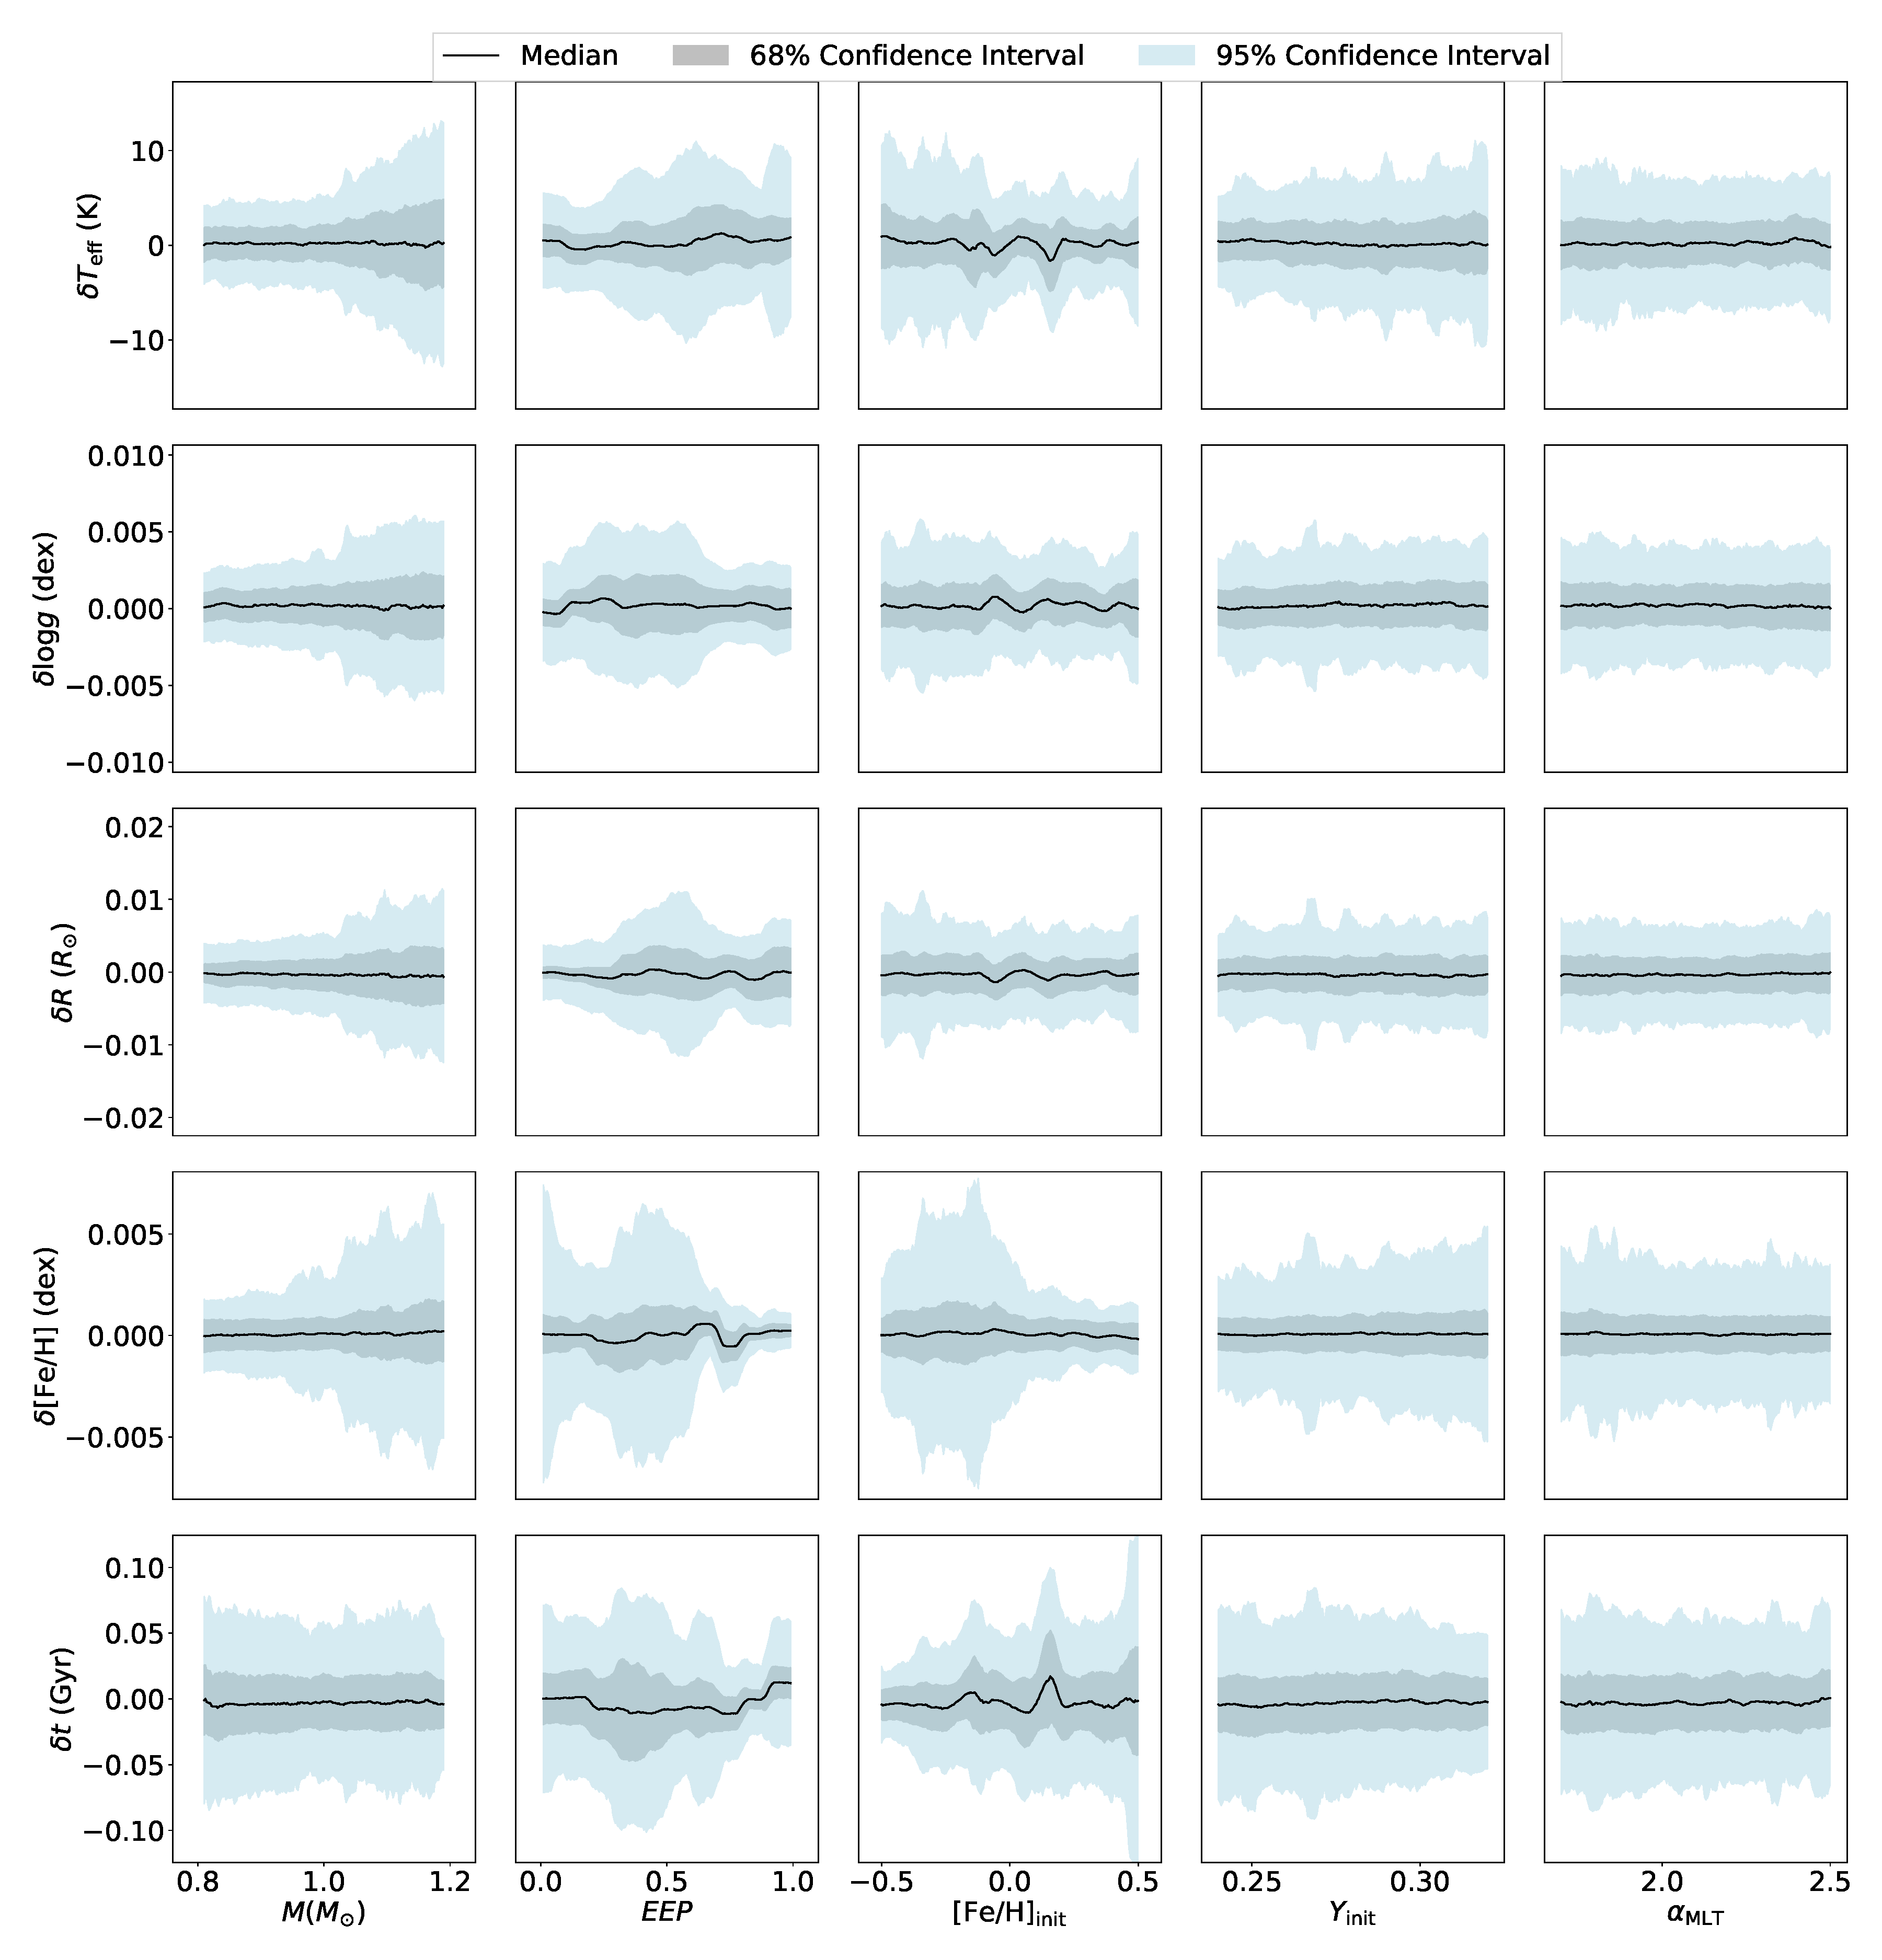
\includegraphics[width=2.0\columnwidth]{ 5d-testing_vs_inputs.pdf}
    \caption{ Roll medians and 68/95\% confidential intervals of testing errors against GP model  inputs. Black solid lines indicate the median value; grey and blue shadowes represent the 68\% and 95\% confidential interval. Testing errors of $T_{\rm eff}$, $\log g$, and $R$ mainly depend on $M$ and{\it EEP}. Metallicity error strongly depends on $M$,{\it EEP}, and {\it [Fe/H]}$_{\rm init}$, and age error has a significant correlation to {\it EEP} and {\it [Fe/H]}$_{\rm init}$. However, testing errors do not obviously relate to $Y_{\rm init}$ or $\alpha_{\rm MLT}$. } 
  \label{fig:5d_test_vs_input}
\end{figure*}
%

\subsection{Mapping Systematic Uncertainties}\label{sec:sys}

A learned GP model predicts output quantities with uncertainties based on its noise model. In our preliminary studies, uncertainties are properly determined for the 1D and 2D problems, but we find obviously underestimated uncertainties in the 3D problem. In the 5D problem, GP models also predict significantly small uncertainties: they are mostly one order of magnitude smaller than testing errors. This is to say, the learned GP models are over-confident for high-demission cases. The reason could be the equally spaced training data, from which GP model learn few variations at the scale smaller than the grid step and hence turns to fit with large lengthscale values.   
% 
Because GP models do not give reliable uncertainties, we intend to use testing errors to estimate the systematic uncertainty in GP prediction. As shown in Figure~\ref{fig:5d_test_vs_input}, systematical uncertainties relate to $M$, {\it EEP}, and {\it [Fe/H]}$_{\rm init}$ but not to $Y_{\rm init}$ or $\alpha_{\rm MLT}$.  We can treat this as a 3D problem and train another GP model, in which GP model systematic uncertainty is a function of $M$, {\it EEP}, and {\it [Fe/H]}$_{\rm init}$. 
%

We inspect the testing errors in the $M$-$EEP$-$\rm {\it [Fe/H]}_{\rm init}$ space and find that their local medians vary smoothly. We hence apply the constant mean function and the RBF kernel. The testing dataset contents 100,000 which exceeds the data size limitation. We use the SVGP approach but not the section scenario for this training, because the SVGP can well handle large data following smooth function (see Appendix \ref{app:B} for detailed discussions about SVGP). 
%
We split the testing error data by 75-to-25 for training and validating.  The variational evidence lower bound (ELBO) is adopted as the loss function because it is designed for when there is too much data for the exact inference. We set up Early Stopping by tracking the RMSE value and terminate training when the RMSE value stops decreasing for 100 iterations. The outputs of GP models are the local medians of testing errors. We use them to infer the systematic uncertainties for five observable quantities (referred as $\sigma_{T_{\rm eff}}$, $\sigma_{\log g}$, $\sigma_{R}$, $\sigma_{\rm {\it [Fe/H]}_{\rm surf}}$, and $\sigma_{\tau}$). To differentiate these GP models, we refer to them as GP-SYS models. In Figure \ref{fig:5d_sys_teff}, we compare the actual local systematic uncertainties for $T_{\rm eff}$ at {\it [Fe/H]}$_{\rm init}$ $\simeq$ 0.0 with those given by the GP-SYS models. It shows that the GP-SYS model well reproduces the $\sigma_{T_{\rm eff}}$ distributions. 

%In the $M$-$EEP$-$\rm {\it [Fe/H]}_{init}$ space, we divide this 3D space into equal-size segments and examine local error distributions. The choice of segment size matters. It needs to be small enough for only presenting the local feature, but it can not be very small so that there are not enough data points for proper statistical analysis. To find an appropriate size, we apply a statistic test. The purpose of the test is to check wether the local distribution has a tail feature. The condition we apply is either the ratio between 68\% and 95\% confidential intervals less than 2.5, or the ratio between 68\% and 99.7\% confidential intervals less than 4. After several attempts, we decide to divide the input range into 40 equally spaced segments for $M$, 50 for {\it EEP}, and 20 for {\it [Fe/H]}$_{\rm init}$. Hence there are 43,911 (41 x 21 x 51) gird points. We compute a rolling standard deviation for each grid point by using the data in a 3-segments (1.5 previous and 1.5 after) range across each demission. The statistic test shows that $\sim90\%$ points meeting the above condition. 
%
%Here the validating errors can be used to examine GP-SYS models. Their average values for all five parameters are small enough to neglect. They are  0.15K for $\sigma_{T_{\rm eff}}$, 0.00008 dex for $\sigma_{\log g}$, 0.0002 $R_{\odot}$ for $\sigma_{R}$, 0.0009 dex for $\sigma_{\rm {\it [Fe/H]}_{\rm surf}}$, and 0.002 Gyr for $\sigma_{\tau}$. 

\begin{figure}
	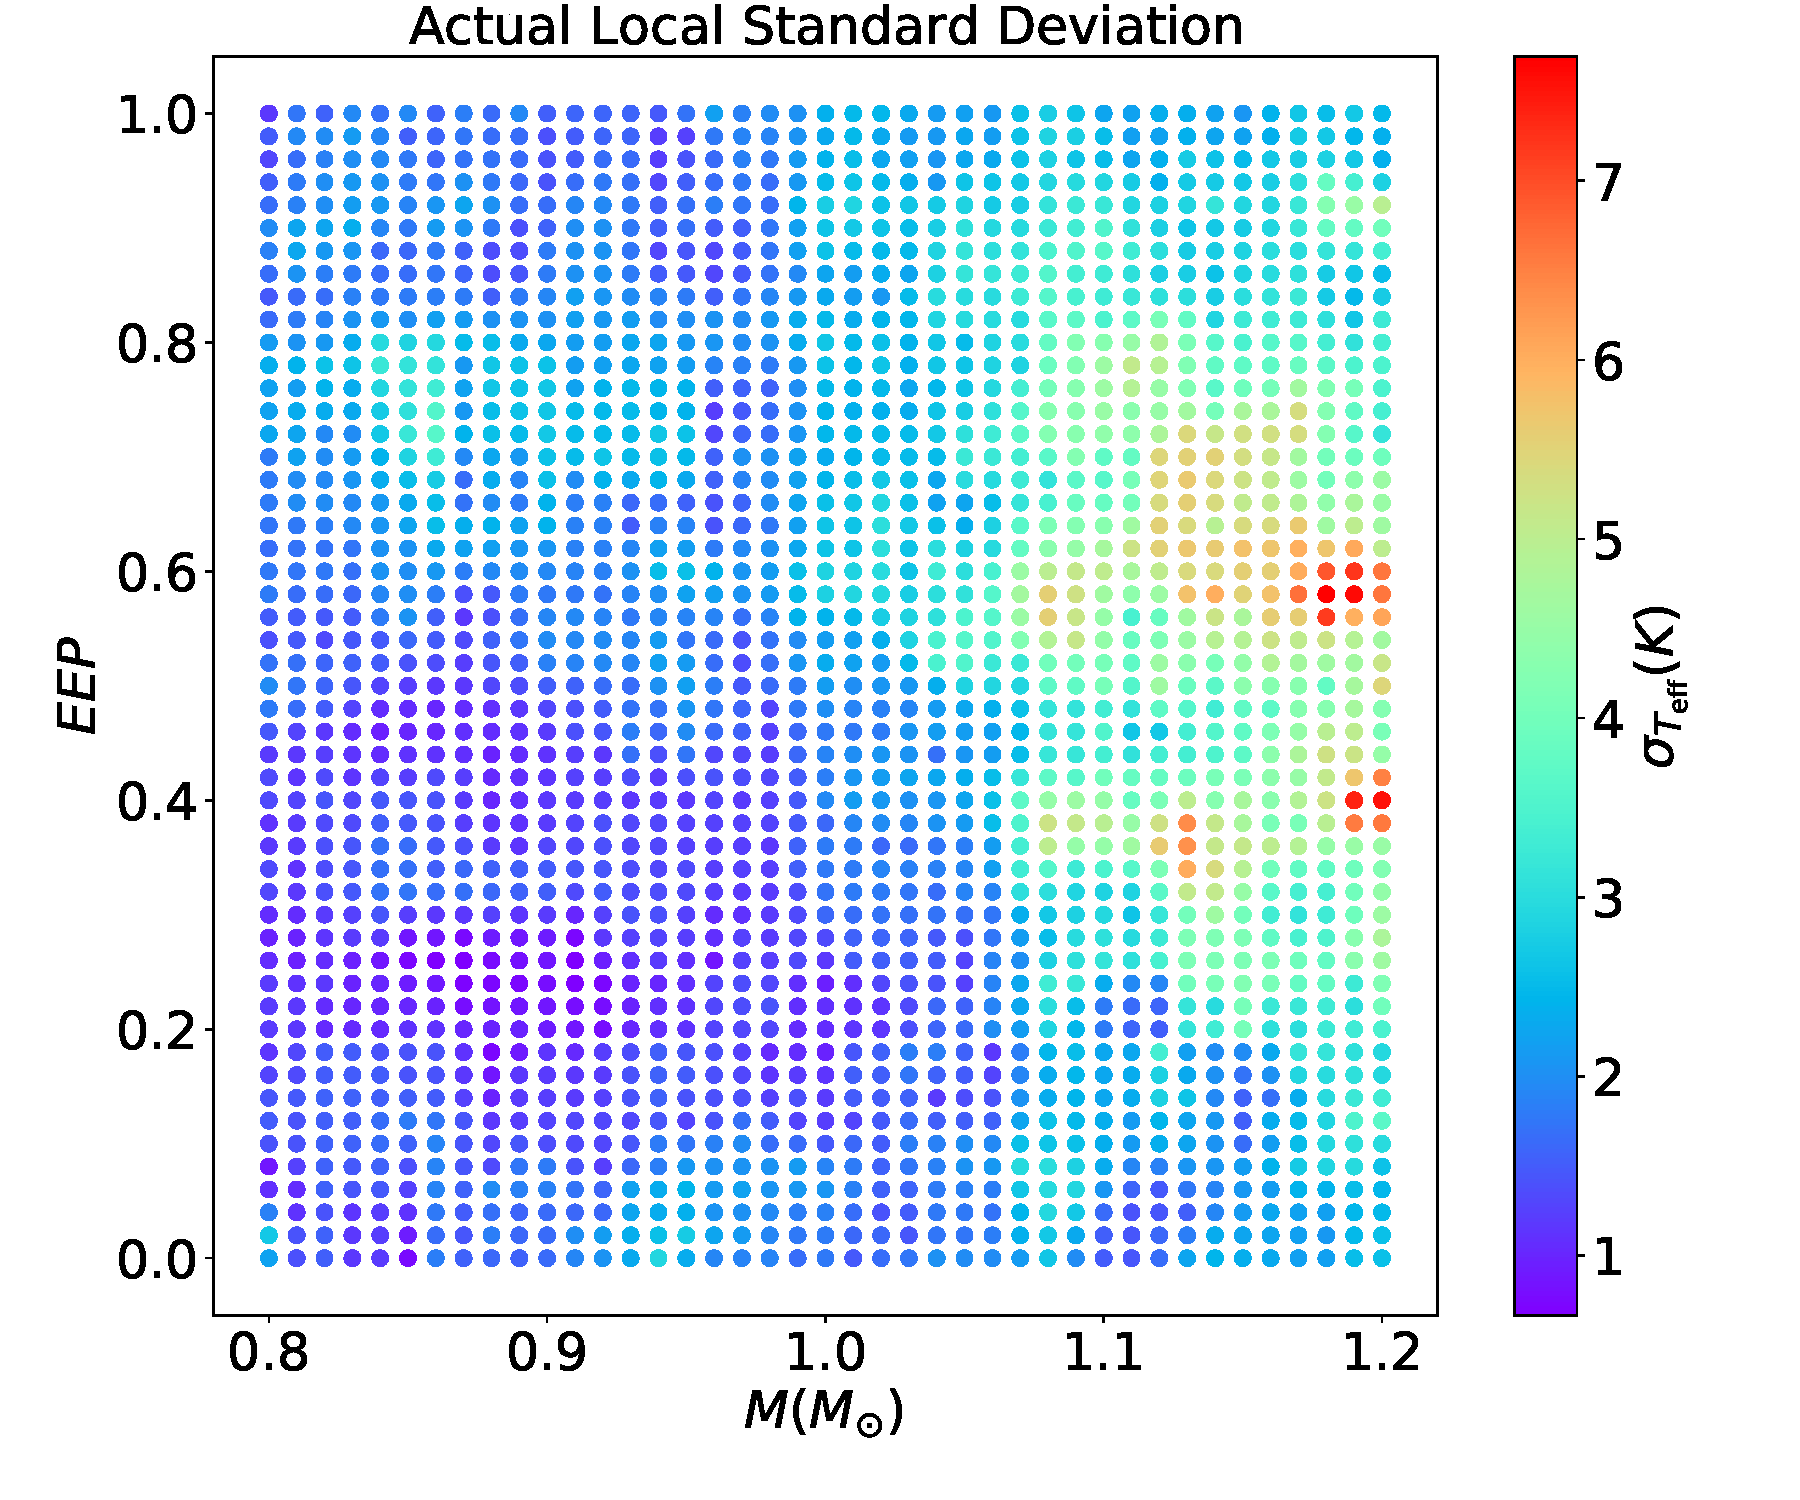
\includegraphics[width=1.0\columnwidth]{5d_sys_teff.pdf}
	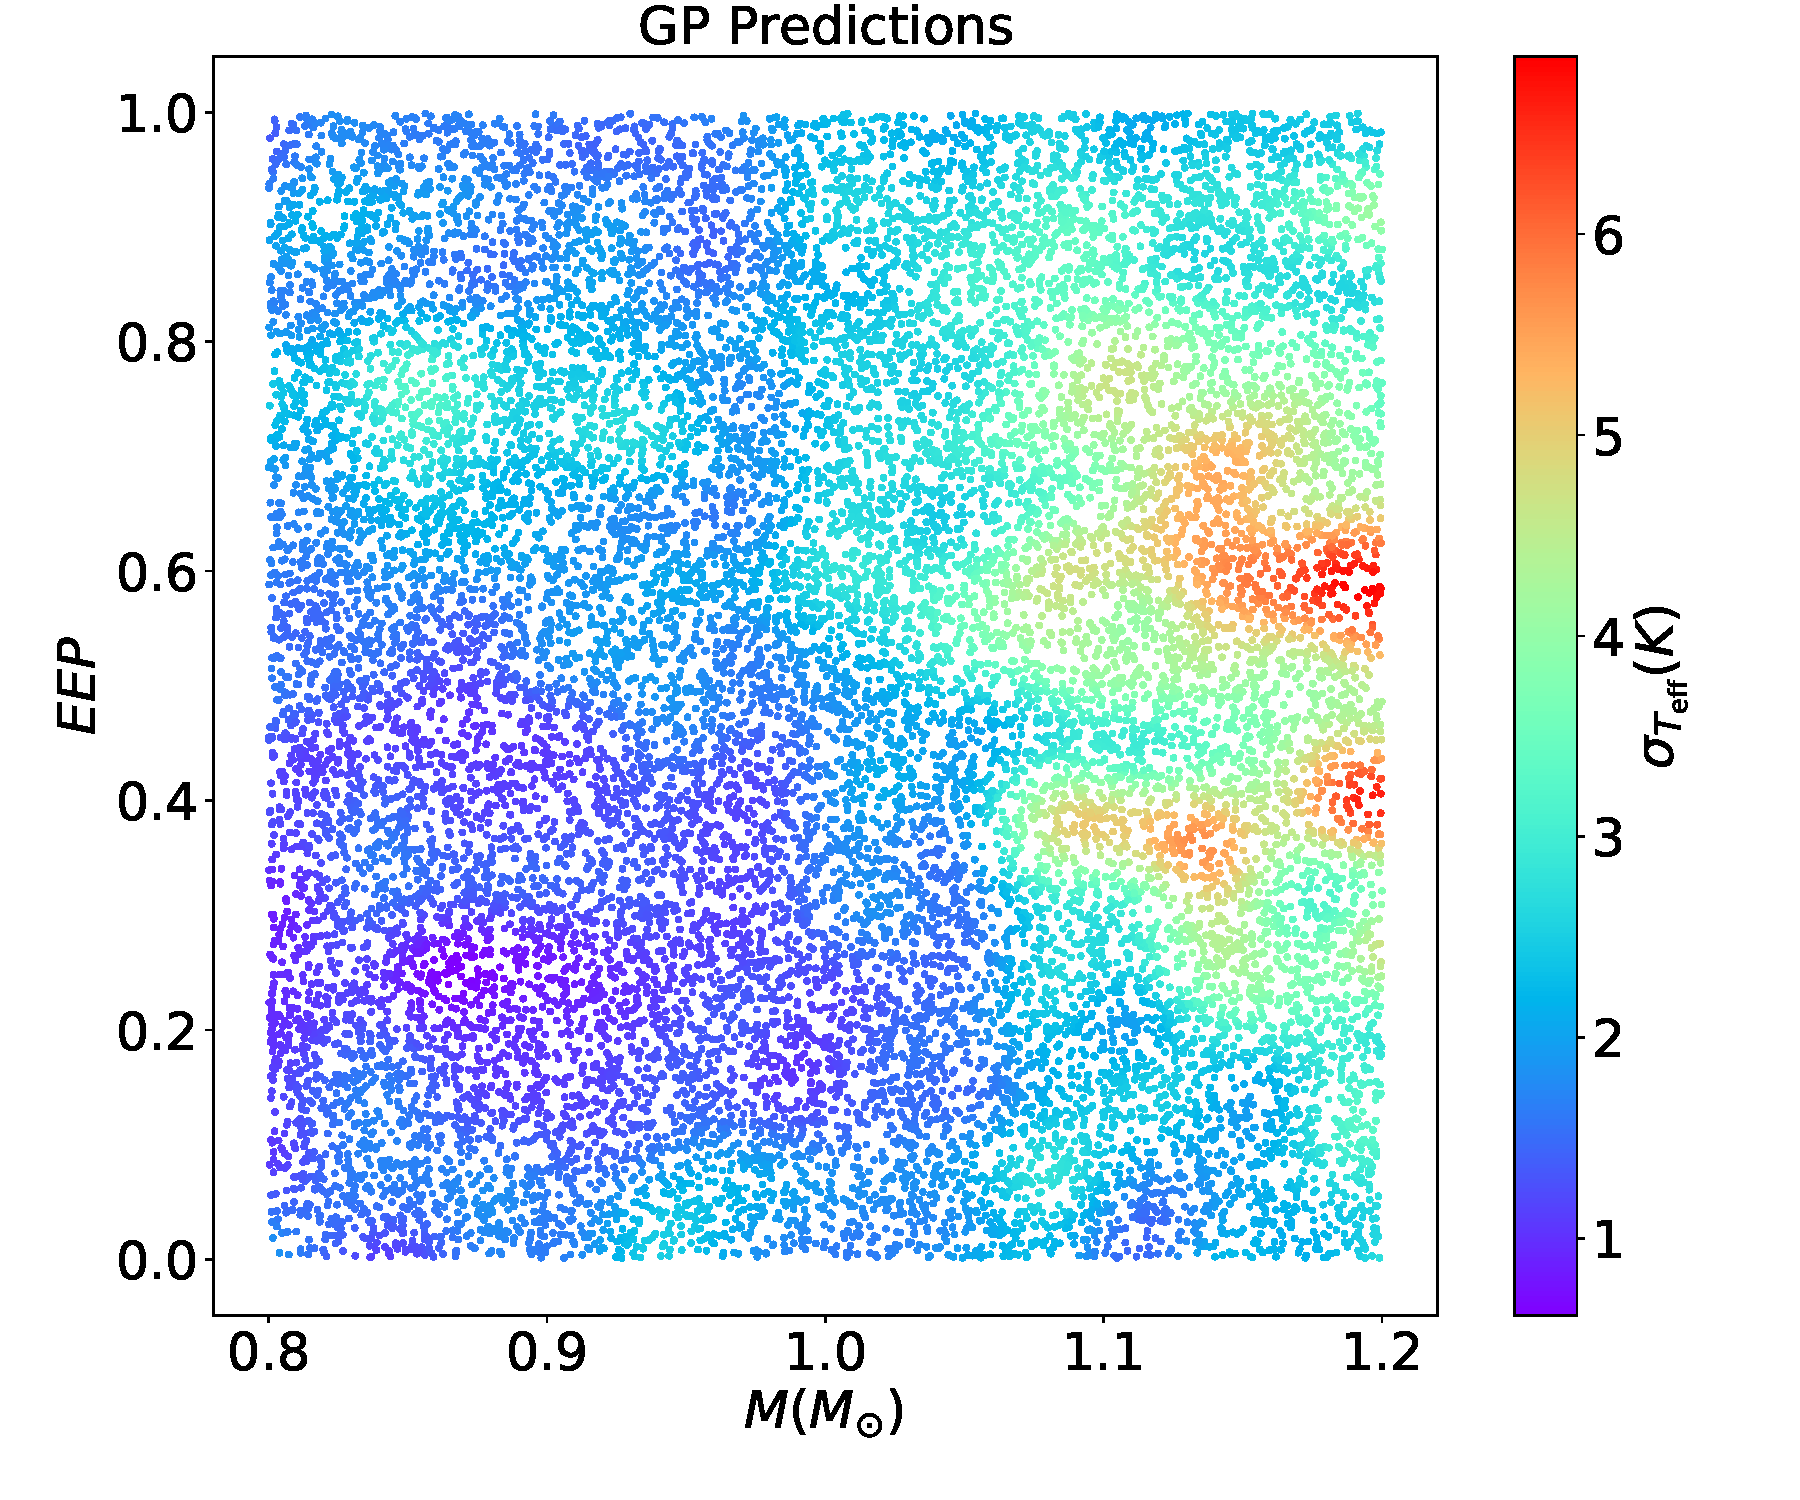
\includegraphics[width=1.0\columnwidth]{5d_sys_effective_T_std_predictions.pdf}
    \caption{Comparison between actual and GP predicted local systematic uncertainties (1-$\sigma$) for $T_{\rm eff}$ on the $M - EEP$ diagram at {\it [Fe/H]}$_{\rm init}$ $\simeq$ 0.0. To calculate the actual local values, we separate the mass range into 40 equally-spaced segments and the {\it EEP} range into 50, and then measure the median testing error for each segment. } 
  \label{fig:5d_sys_teff}
\end{figure}

%\begin{table}
%	\centering
%	\caption{Residual of GP models for systematic uncertainty}
%	\label{tab:sys}
%	\begin{tabular}{lc}
%		\hline
%		GP output& Average Validating Errors (ABS) \\
%		\hline
%		$\sigma_{T_{\rm eff}}$  (K) & 0.15 \\
%		$\sigma_{\log g}$  ($10^{-3}$dex)   & 0.08 \\
%		$\sigma_{R}$ ($10^{-3}R_{\odot}$)   & 0.2 \\
%		$\sigma_{\rm {\it [Fe/H]}_{\rm surf}}$ ($10^{-3}$dex) & 0.09 \\
%		$\sigma_{\tau}$ ($10^{-2}$ Gyr)  & 0.2\\
%		%$\sigma_{\Delta\nu} (\mu Hz)$ & 0.01\\
%		  \hline
%	\end{tabular}
%\end{table}


\section{Modelling stars with GP predictions}\label{sec:augmentation}


\subsection{Augmenting the model grid}

Now we are able to use learned GP models to augment the original stellar grid. We randomly sample 5,000,000 data points with uniform distributions for five fundamental inputs ($M$, {\it EEP}, {\it [Fe/H]}$_{\rm init}$, $Y_{\rm init}$, and $\alpha_{\rm MLT}$). We then predict output quantities using GP models and their systematic uncertainties using GP-SYS models. This GP-based model dataset can be downloaded following the instruction at \url{https://github.com/litanda/GPGird}. In Figure~\ref{fig:5d_augmentation}, we demonstrate the original grid, GP predictions, and GP systematic uncertainties on the Kiel diagram. 

\begin{figure*}
	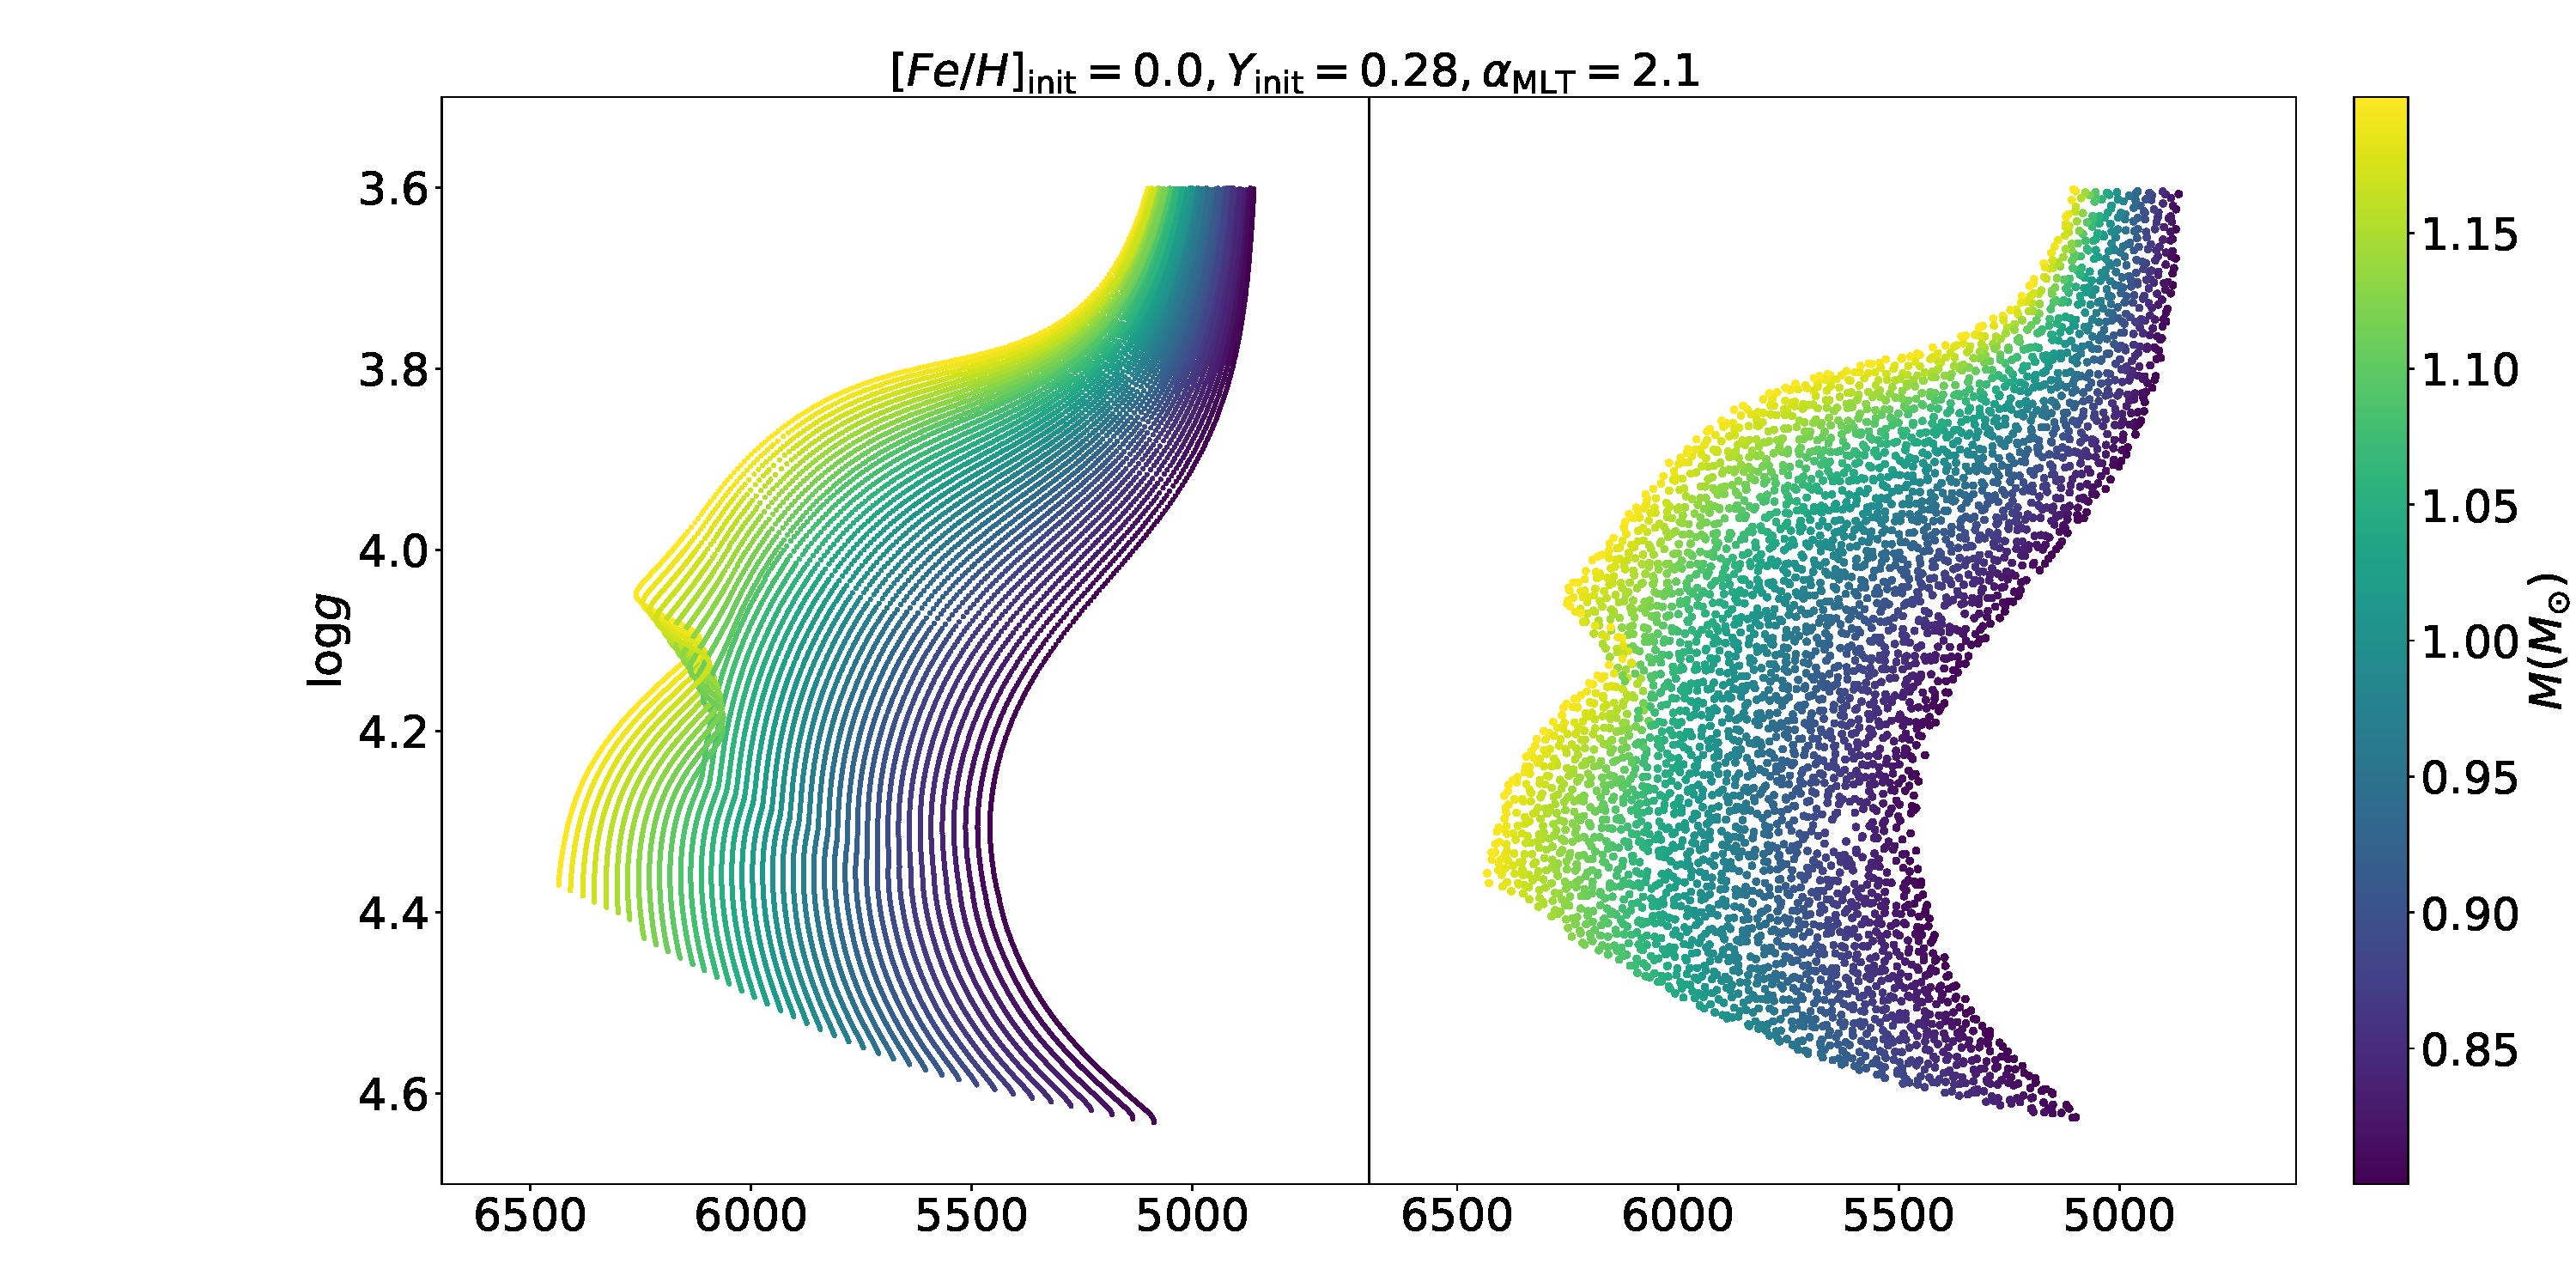
\includegraphics[width=1.3\columnwidth]{5d-au-mass.pdf}
	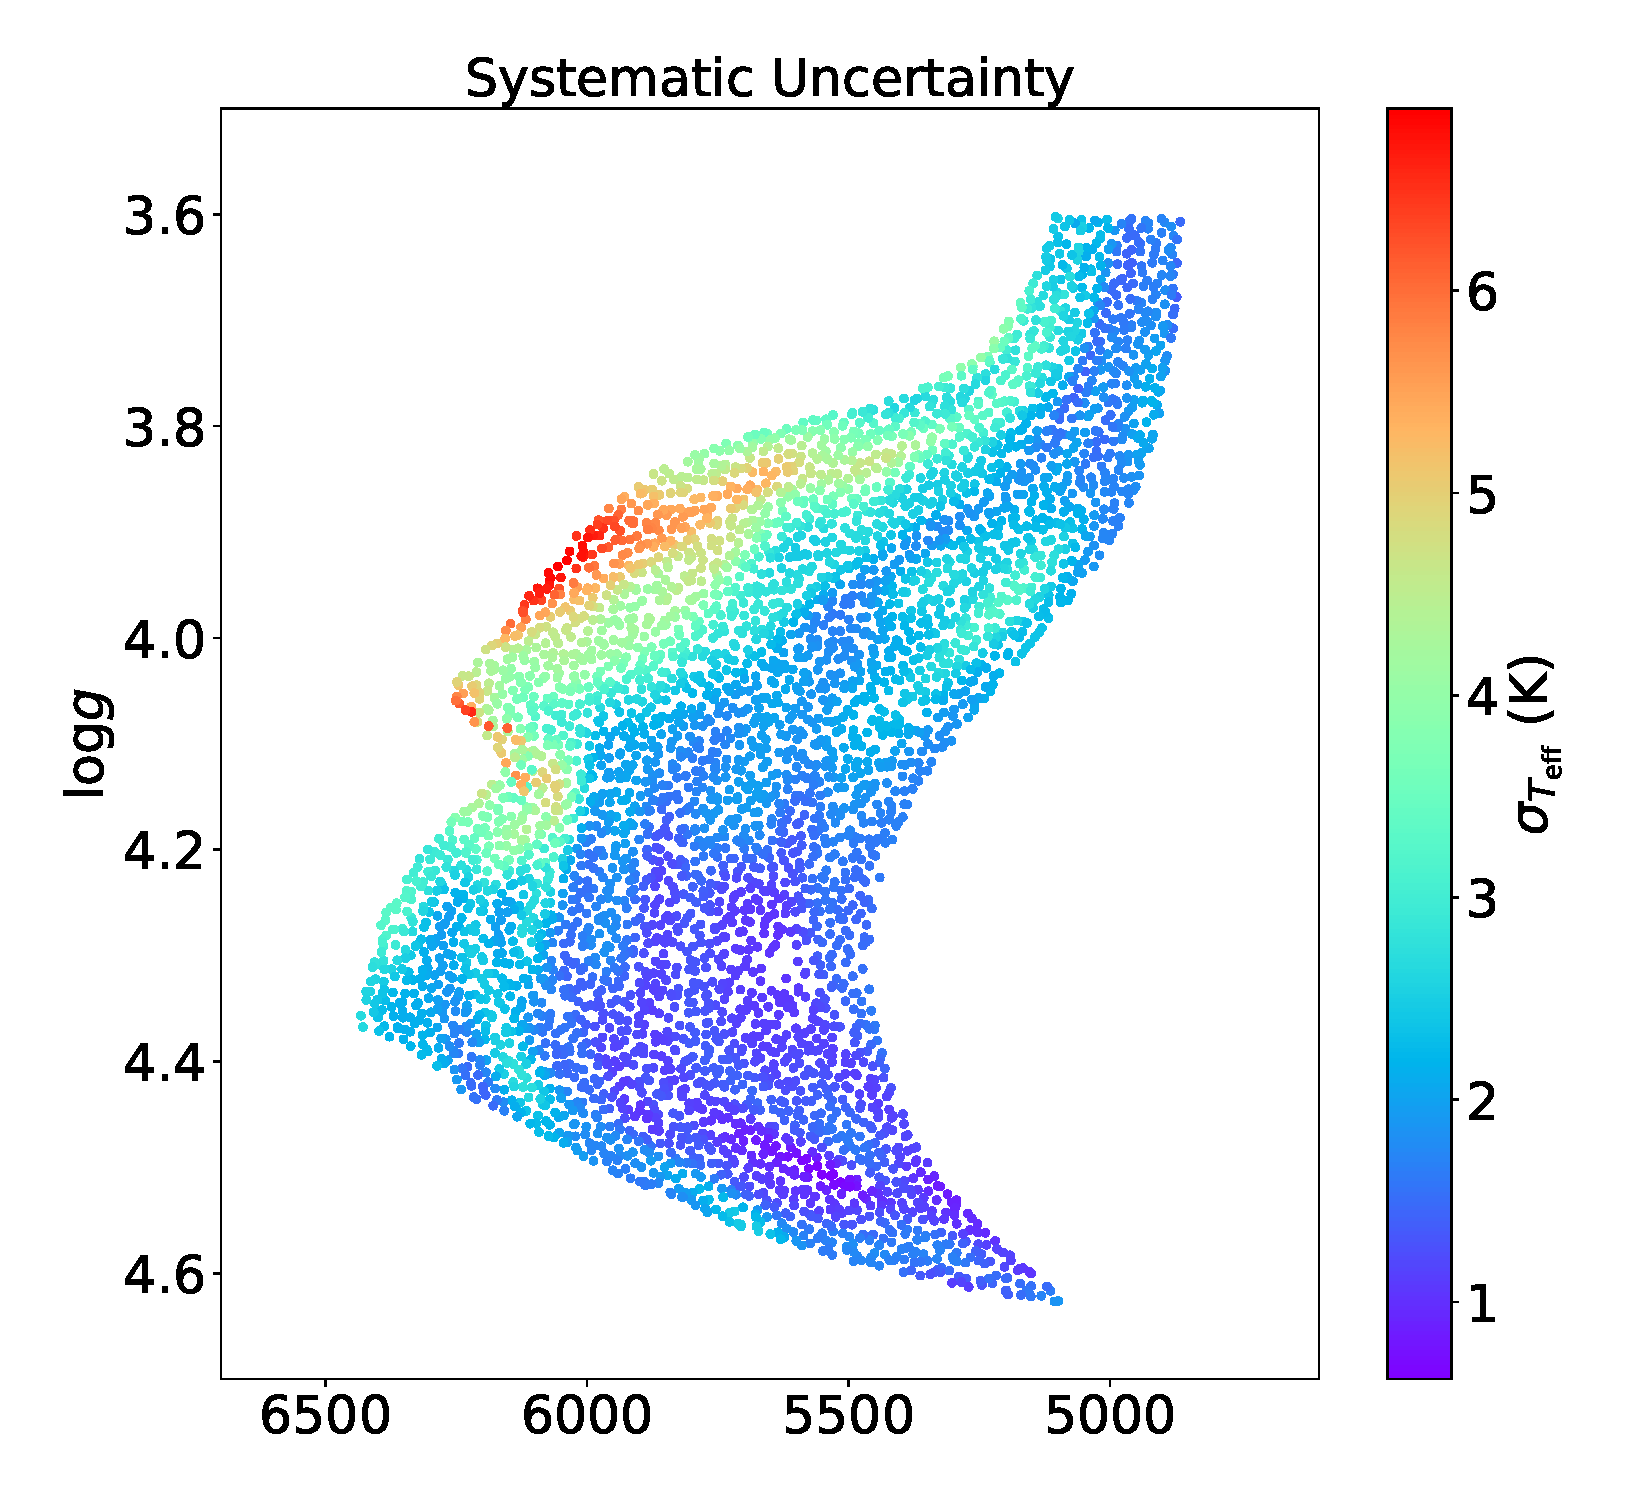
\includegraphics[width=0.7\columnwidth]{5d-au-mass-sys.pdf}
	%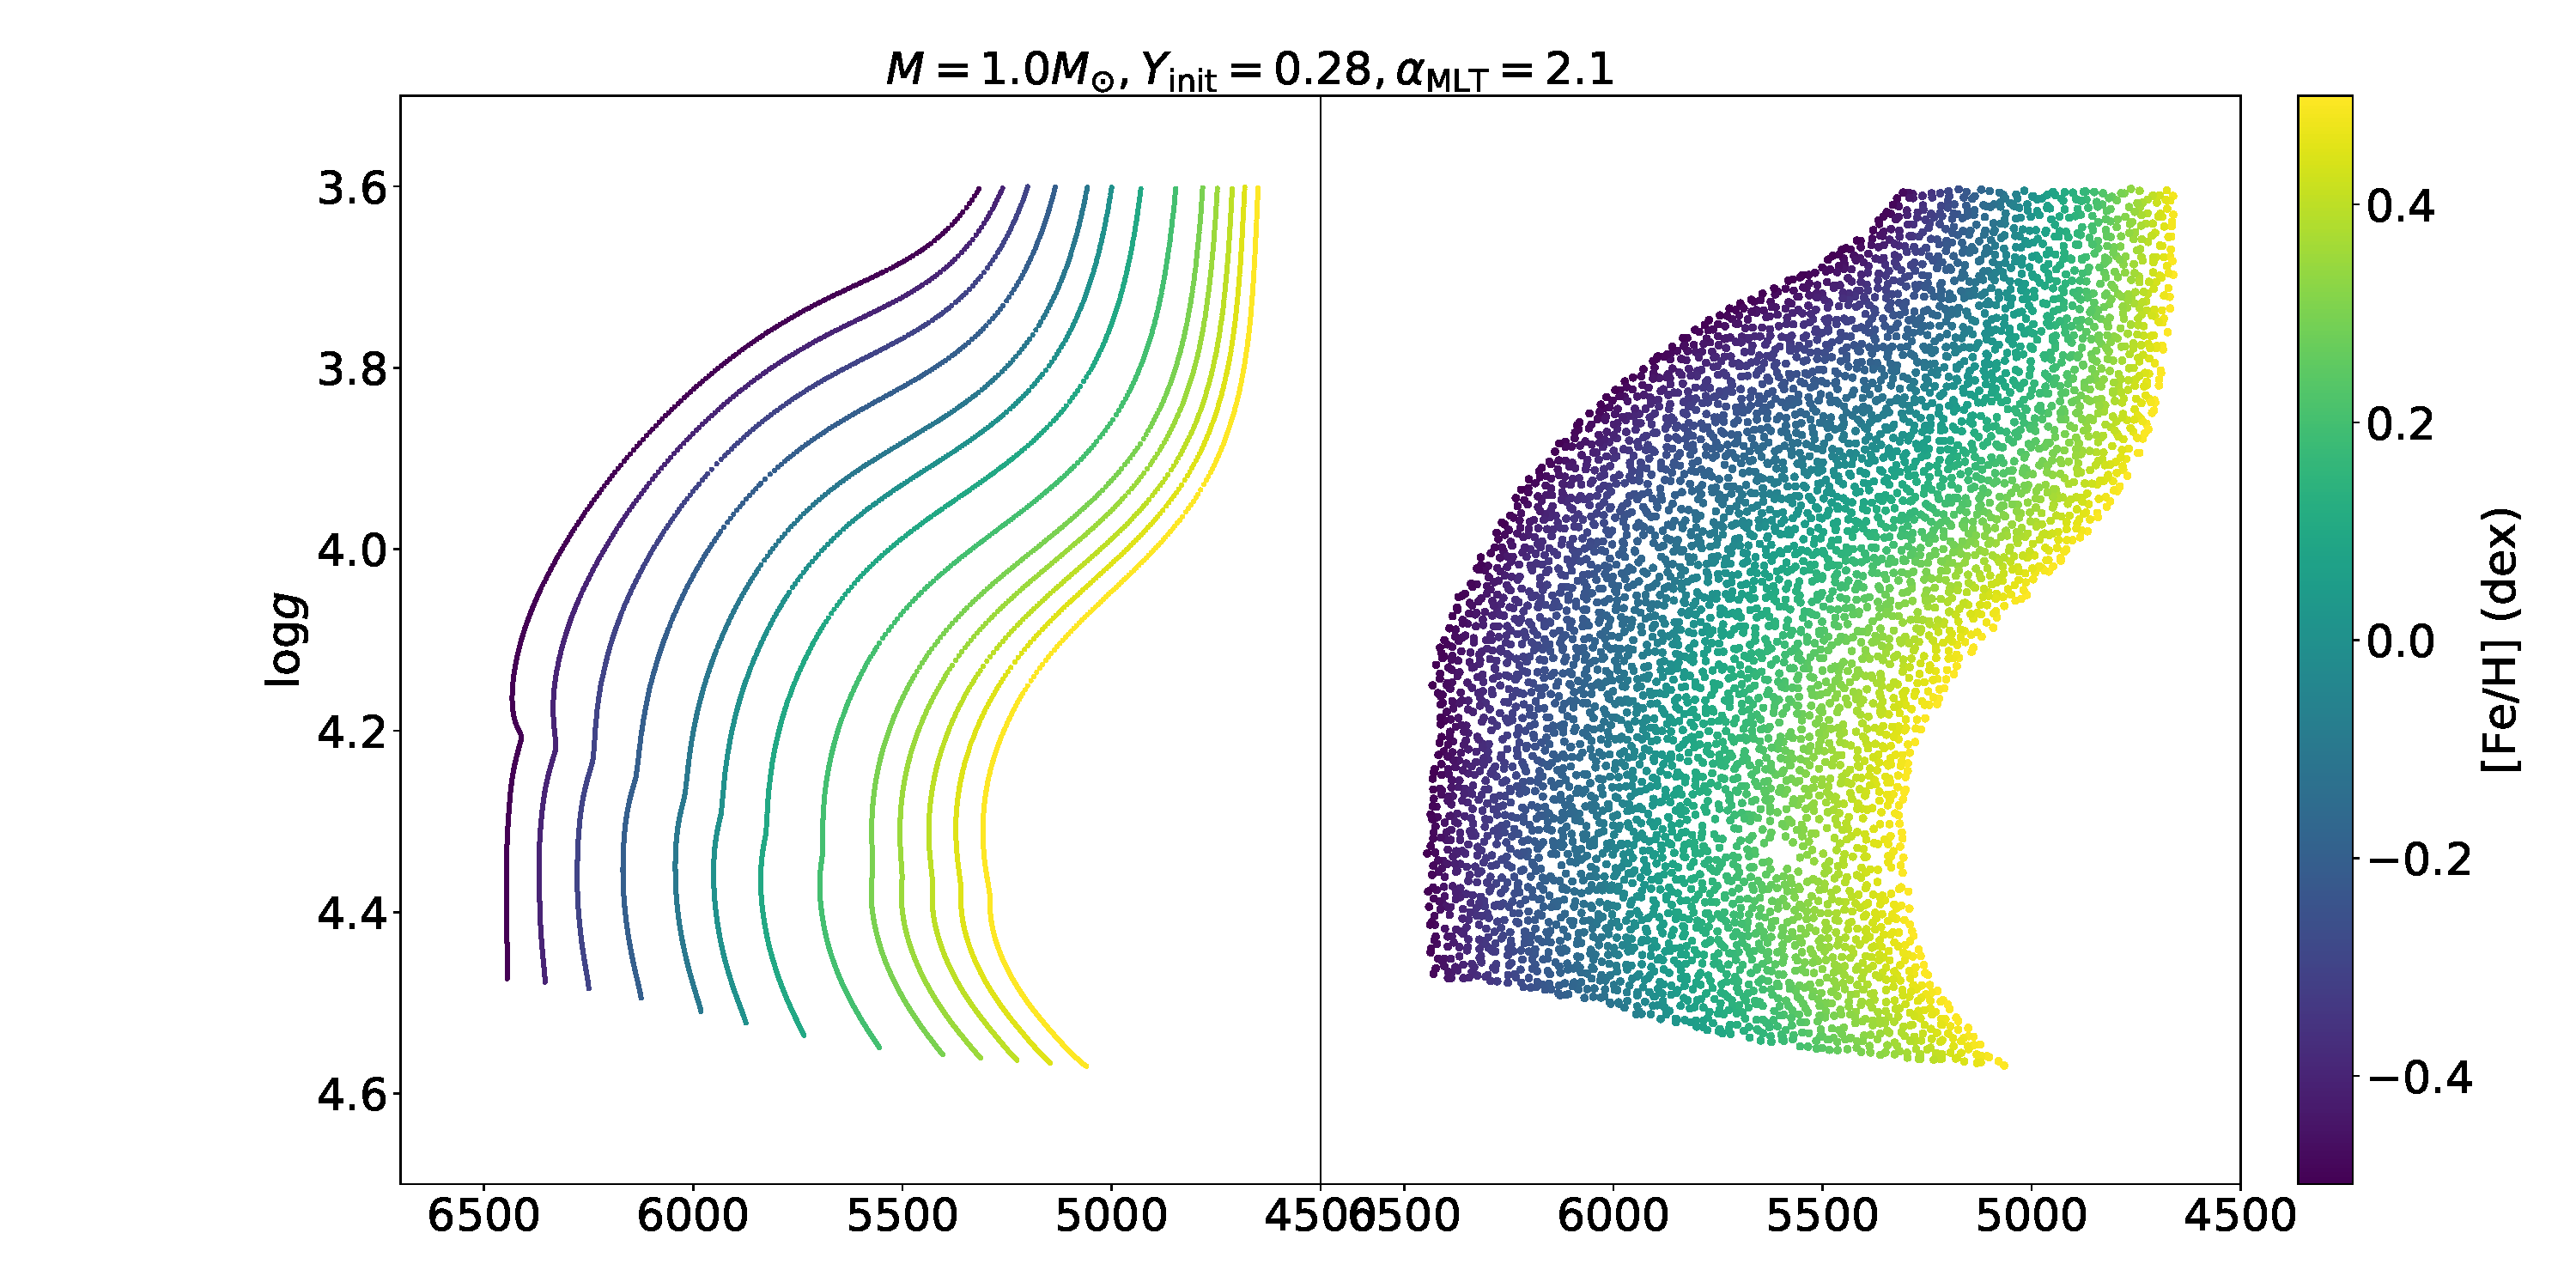
\includegraphics[width=1.2\columnwidth]{5d-au-feh.pdf}
	%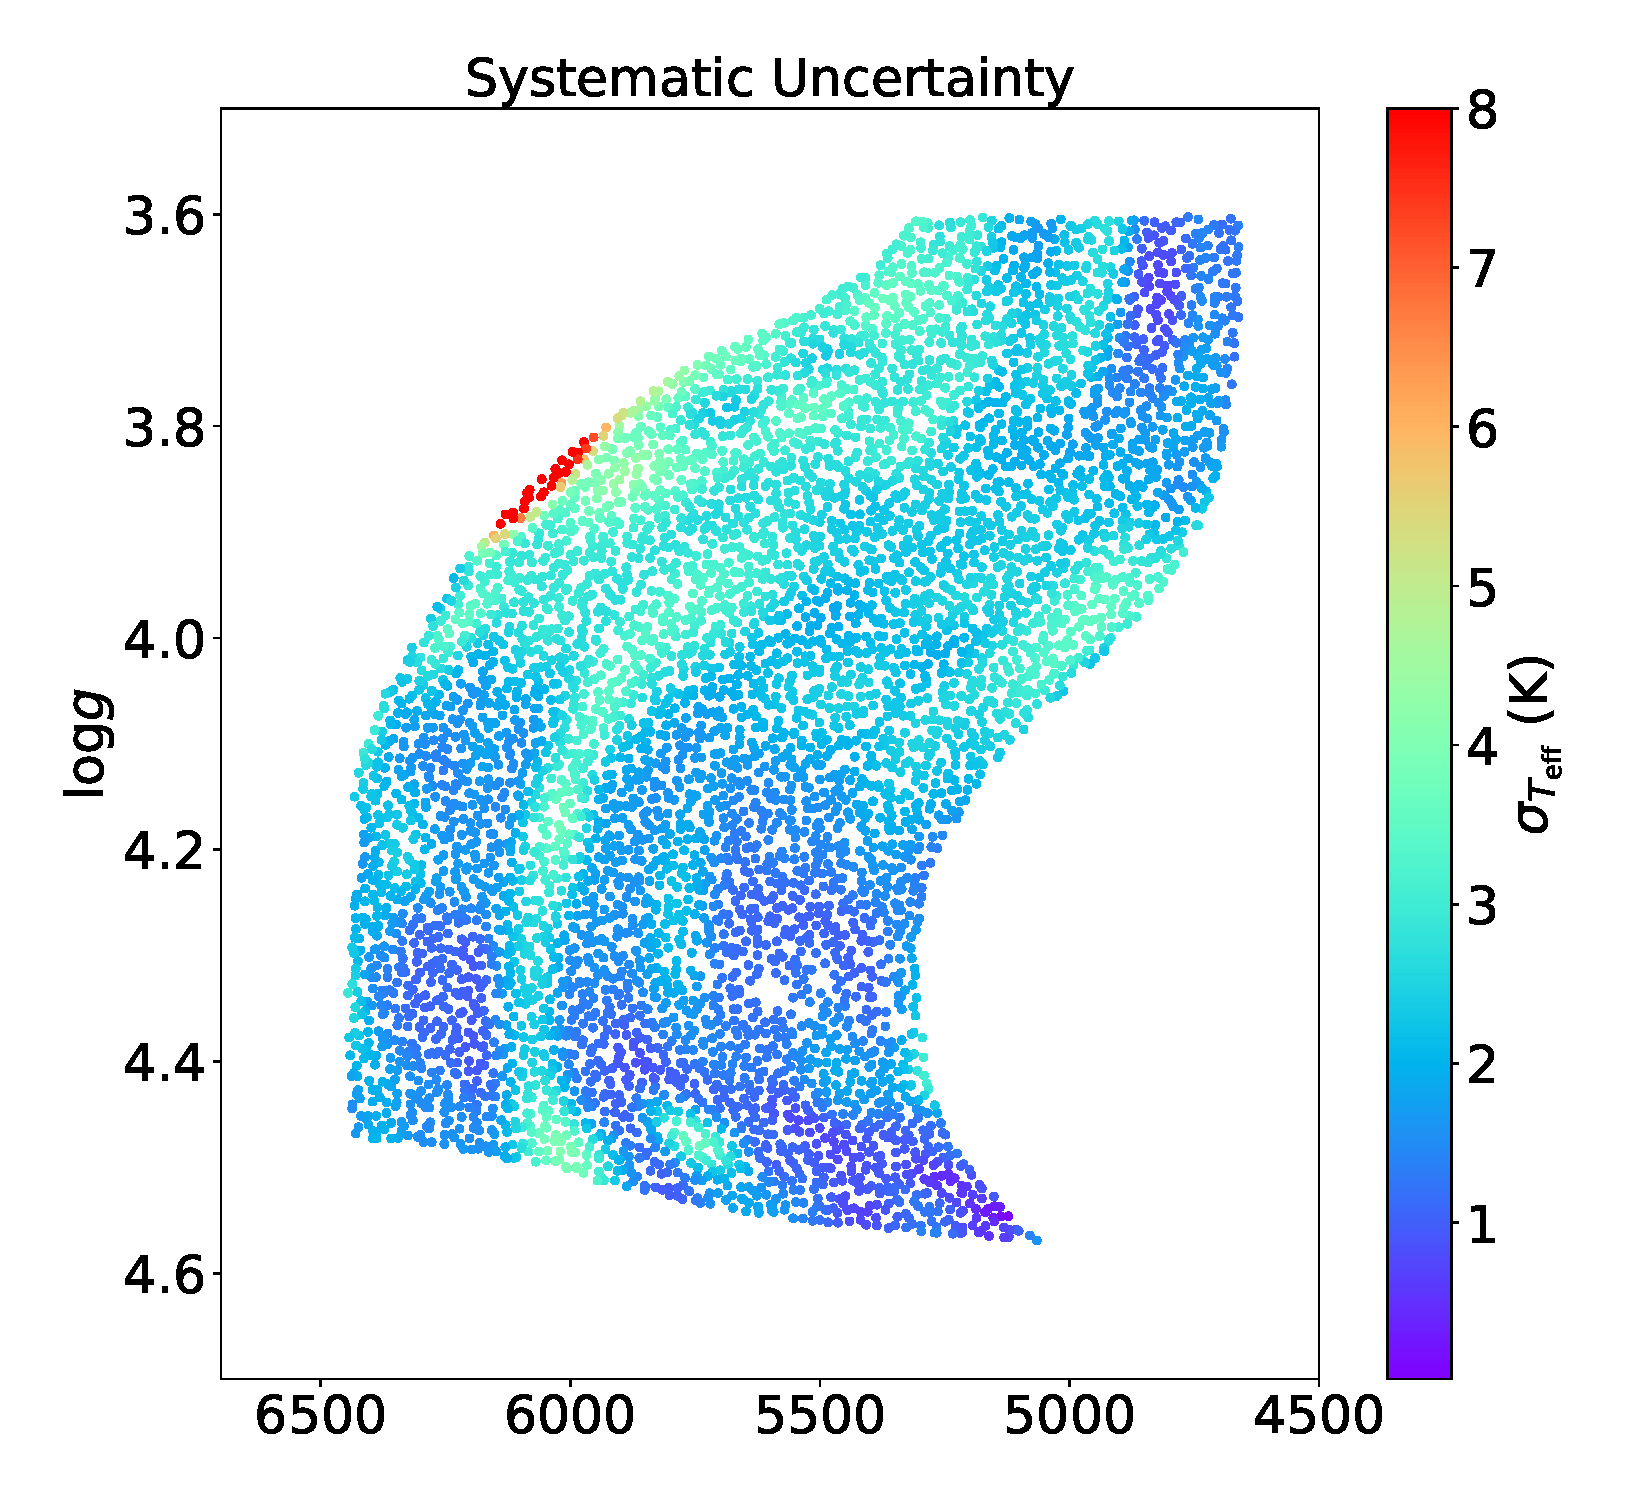
\includegraphics[width=0.65\columnwidth]{5d-au-feh-sys.pdf}
	%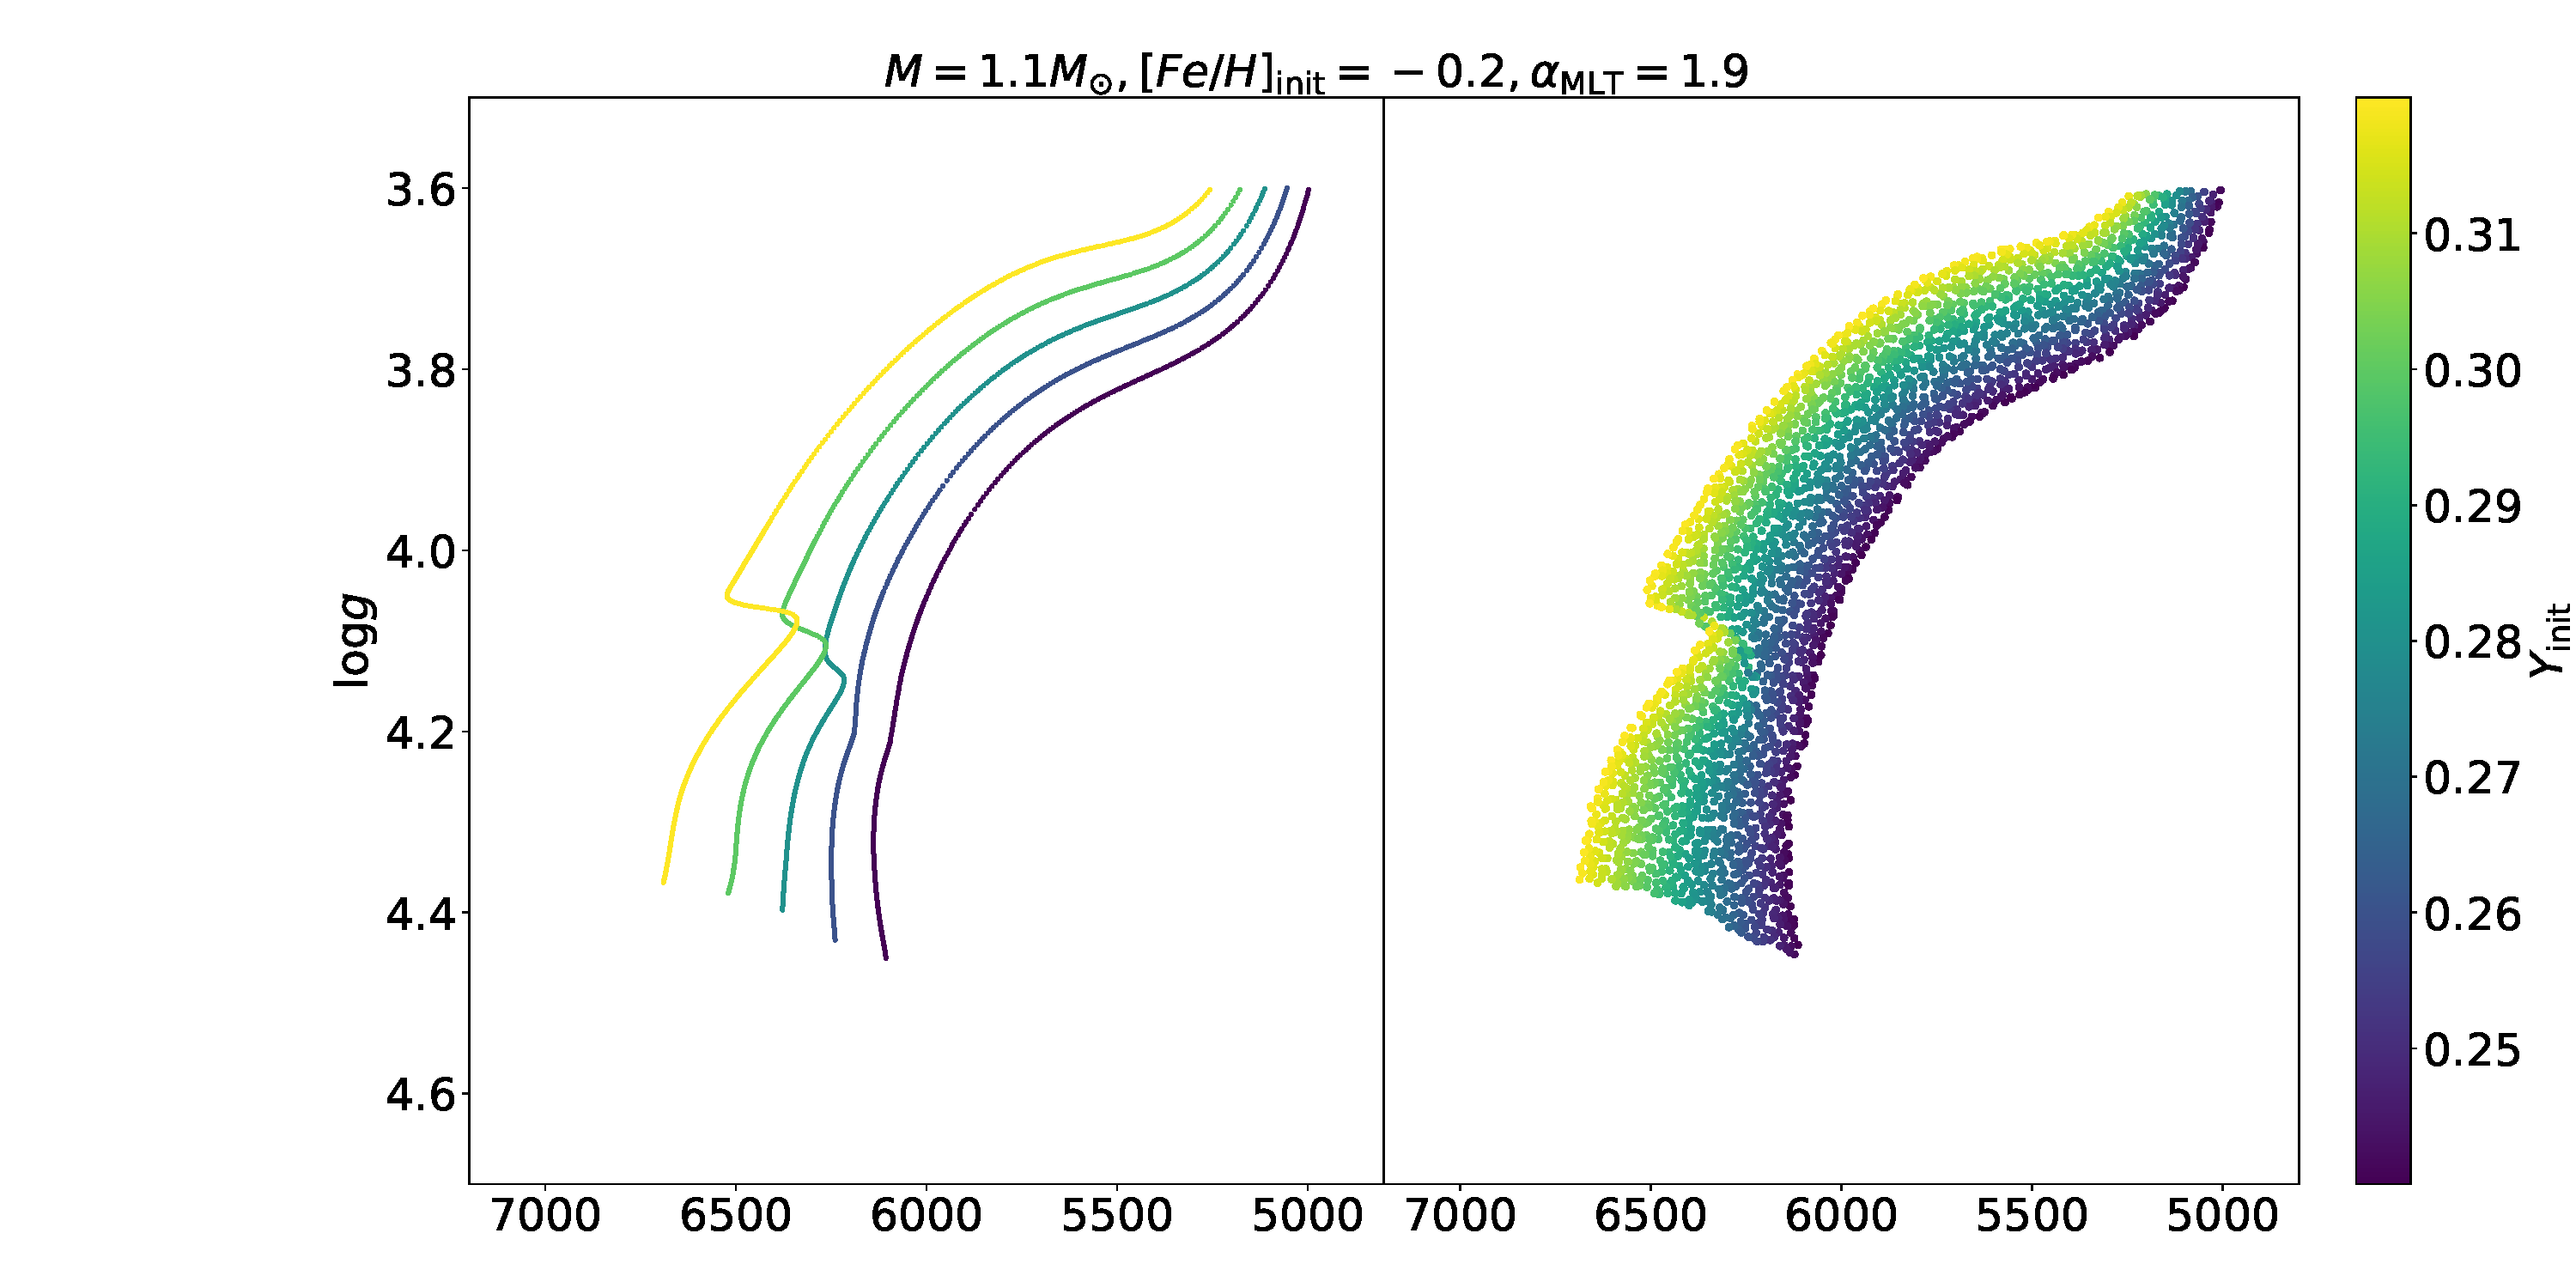
\includegraphics[width=1.2\columnwidth]{5d-au-y.pdf}
	%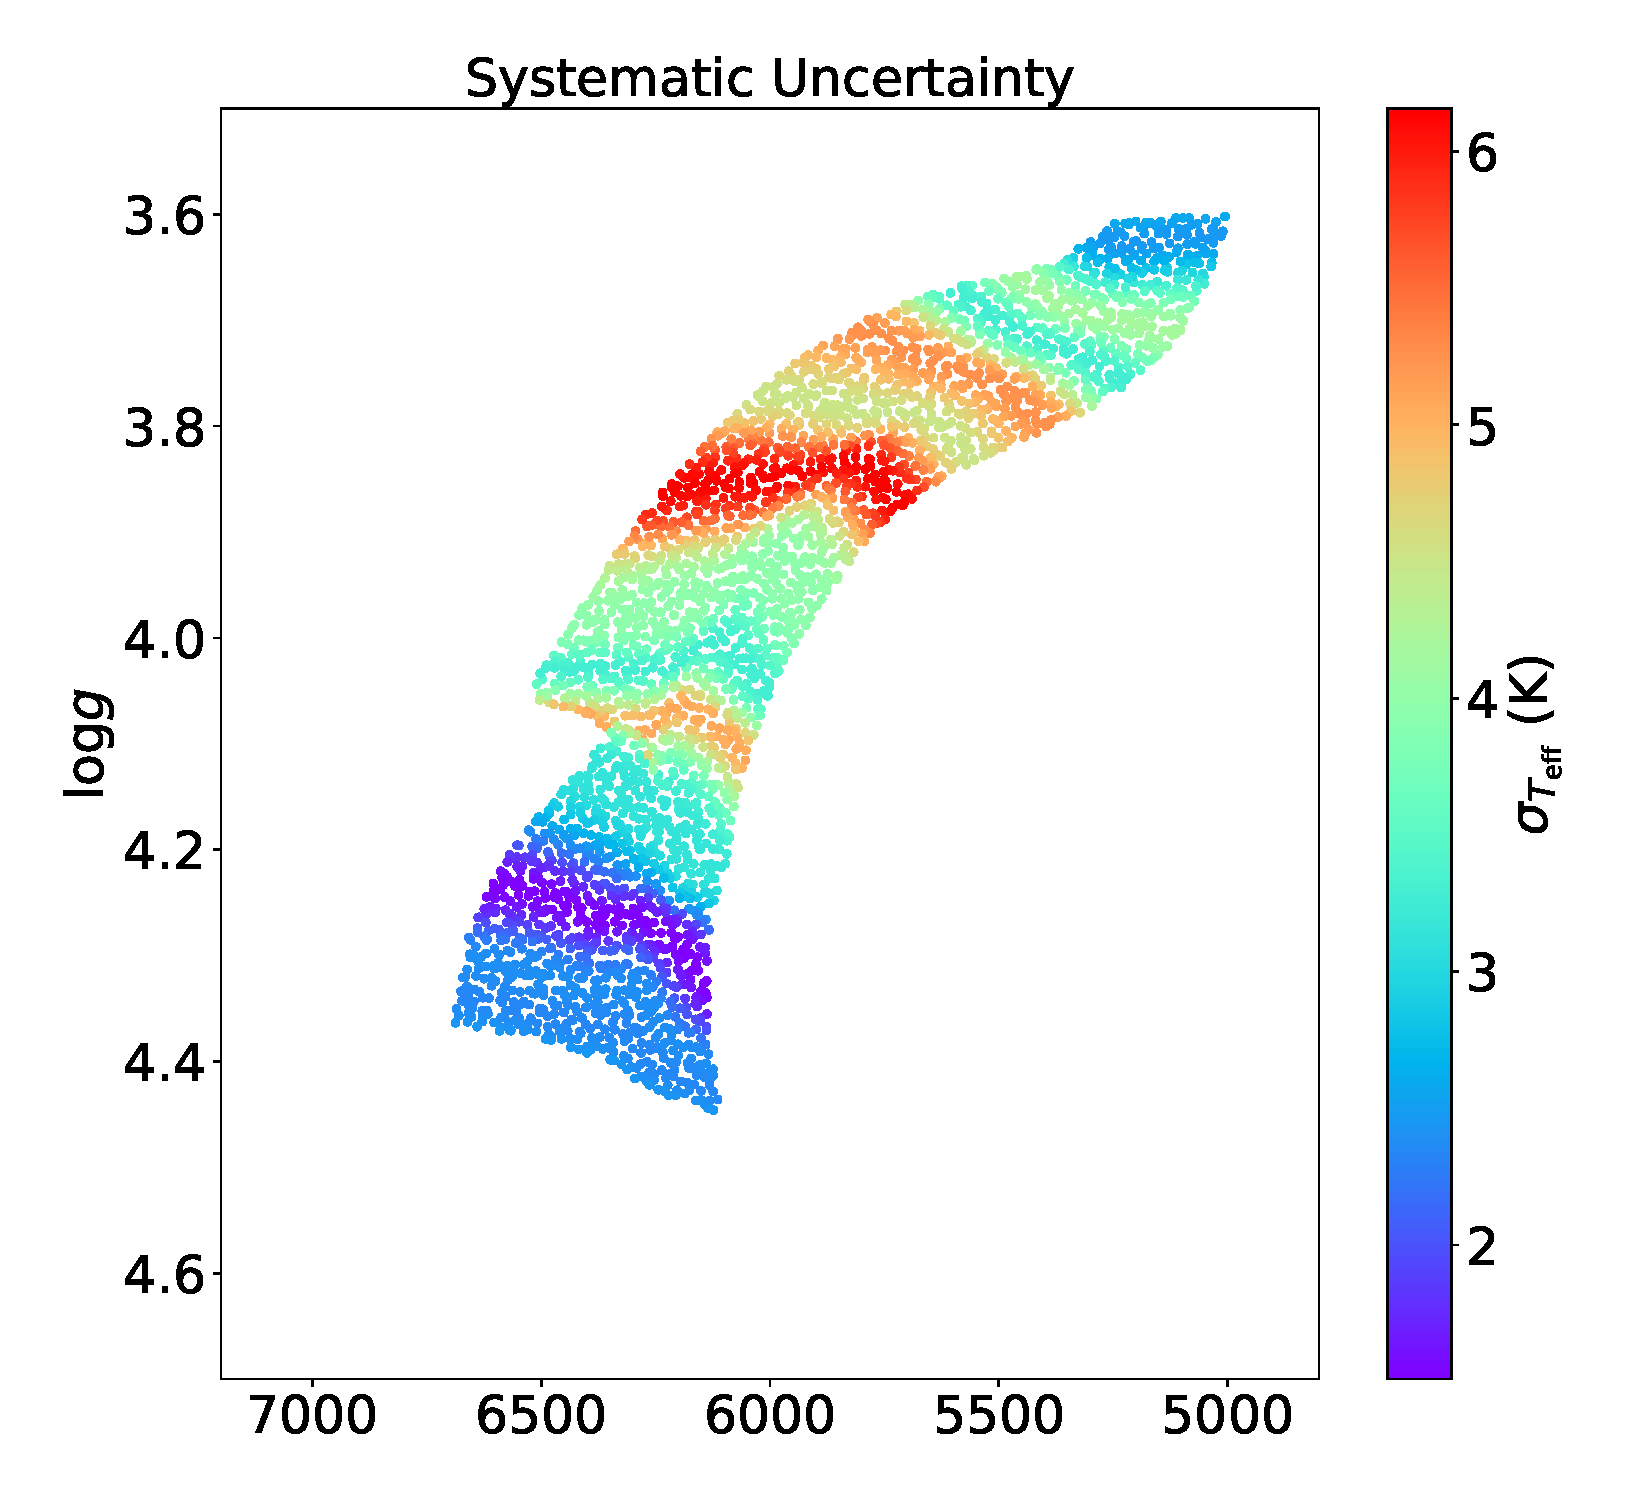
\includegraphics[width=0.65\columnwidth]{5d-au-y-sys.pdf}
	%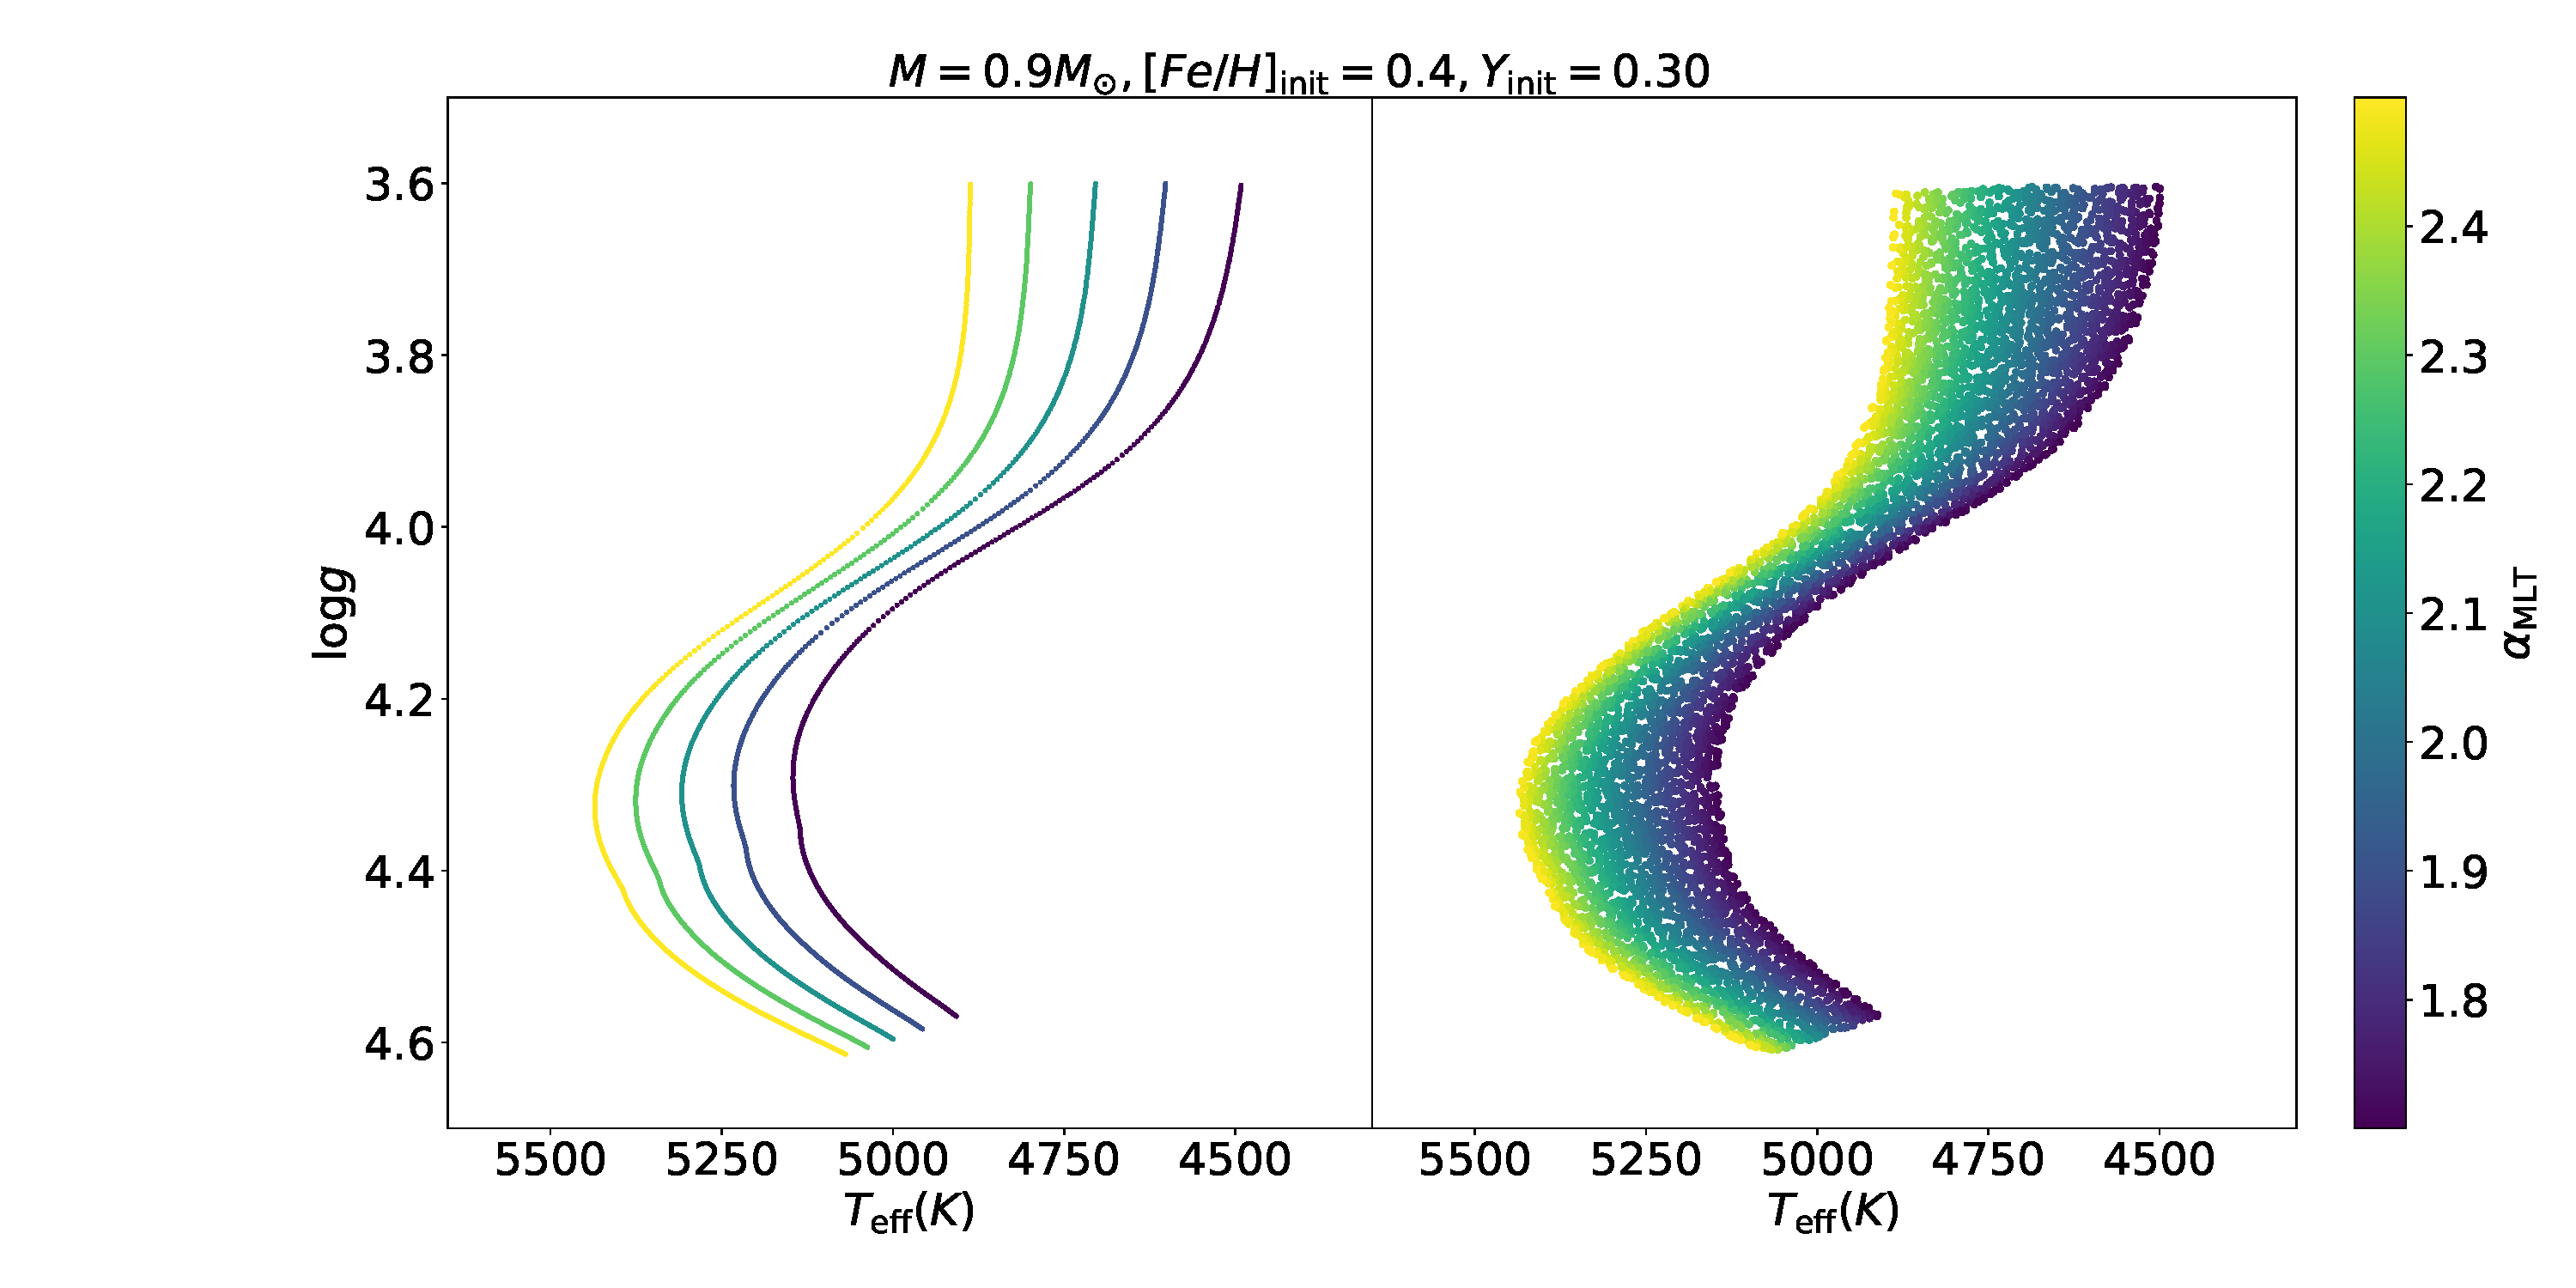
\includegraphics[width=1.2\columnwidth]{5d-au-alpha.pdf}
	%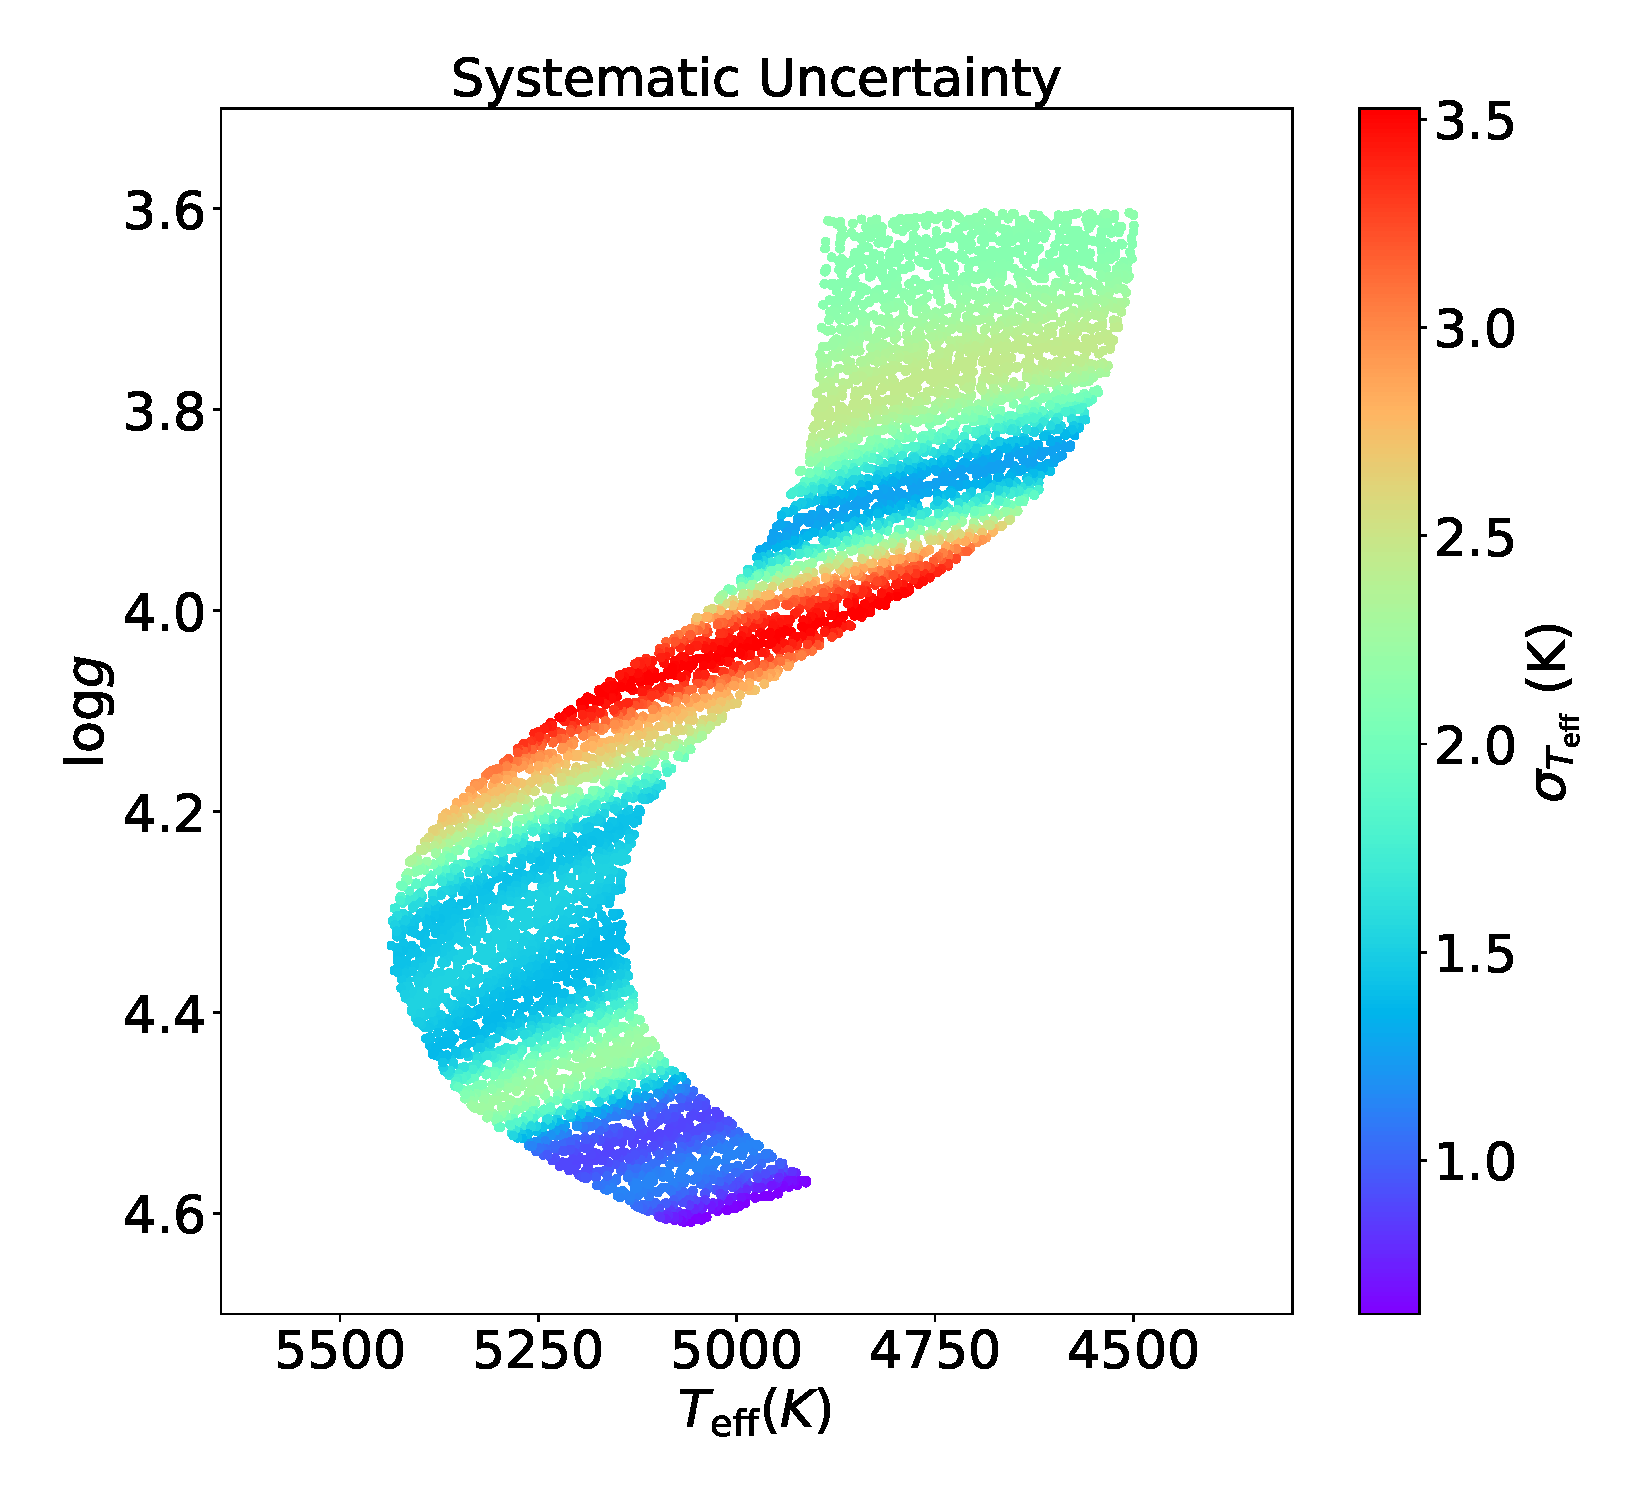
\includegraphics[width=0.65\columnwidth]{5d-au-alpha-sys.pdf}
    \caption{ Left: Comparing the original grid and GP predictions on Kiel diagram. Right: The systematical uncertainties for $T_{\rm eff}$ given by GP-SYS models.} 
  \label{fig:5d_augmentation}
\end{figure*}


\subsection{GP-based Modelling for 1,000 Fake Stars}

As a final test of our method, we use GP-predicted stellar models to characterise 1,000 fake stars to examine whether the method recovers true stellar properties. 
We compute 1,000 fake model stars with the same input physics as the grid but randomly sampled input fundamental parameters. To avoid the edge effect, fake stars are computed in the range of $T_{\rm eff}$ = [4700K, 6800K], $\log g$ = [3.7, 4.6], {\it [Fe/H]}$_{\rm surf}$ = [-0.35,0.35], $M$ = [0.85,1.15], {\it EEP} = [0.05,0.95], $Y_{\rm init}$ = [0.25,0.31], and $\alpha_{\rm MLT}$ = [1.8,2.4].
%
We use four observables, i.e., $T_{\rm eff}$, $\log g$, $R$, and {\it [Fe/H]}$_{\rm surf}$, as observed constraints. We apply typical observed uncertainty that is $\pm$50K for $T_{\rm eff}$ (high-resolution spectroscopy), $\pm0.005$dex for $\log g$ (seismology), $3\%$ for $R$ (seismology), and $\pm0.05$dex for {\it [Fe/H]}$_{\rm surf}$ (high-resolution spectroscopy). Observed value for each constraint is calculated with true value plus a random noise which follows a Gaussian distribution.  

We fit fake stars using the Maximum Likelihood Estimate (MLE) method. Note that the variance term in the MLE function contents observed uncertinaty and also the model systematic uncertainty determined with GP-SYS models ($\sigma^{2} = \sigma_{obs}^{2} +  \sigma_{sys}^{2} $). We measure the 16th, 50th, and 84th percentiles of the likelihood distribution to estimate a parameter and its uncertainty. 


We present inferred stellar parameters for a representative fake star in Figure \ref{fig:fit_comparison}. Observed constraints for this fake star are $T_{\rm eff}$ = 5652$\pm$50K, $\log g$ = 4.424$\pm$0.005, {\it [Fe/H]}$_{\rm surf}$ =  0.31$\pm$0.05, and $R$ =  1.047$\pm$0.031$R_{\odot}$. True fundamental parameters are $M$ = 1.062$\rm M_{\odot}$, $\tau$ = 3.79Gyr, $\rm {\it [Fe/H]}_{init}$ = 0.364, $Y_{\rm init}$ = 0.292, and $\alpha_{\rm MLT}$ = 1.984 (blue dashes). We fit with both the original model grid and the GP predictions for comparing.
%
As it shown that the GP-based modelling has a completed statistical sampling and hence gives more sensible posterior distributions than the grid-based modelling. The improvement for the age is obvious. GP-based modelling infers an age of $4.3^{+2.0}_{-1.8}$Gyr, which is more accurate and precise than that determined with the original grid ($4.4^{+2.2}_{-2.4}$Gyr). The age estimate with the original grid does not actually converge because of under sampling. For initial metallicity, initial helium fraction, and the mixing-length parameter, GP-based models make it possible to properly estimate them without computing a very fine model grid. Thus, GP is an efficient tool to augment a typical stellar model grid and overcome the under sampling issue, as a result, improves the precision of estimate.  

\begin{figure*}
	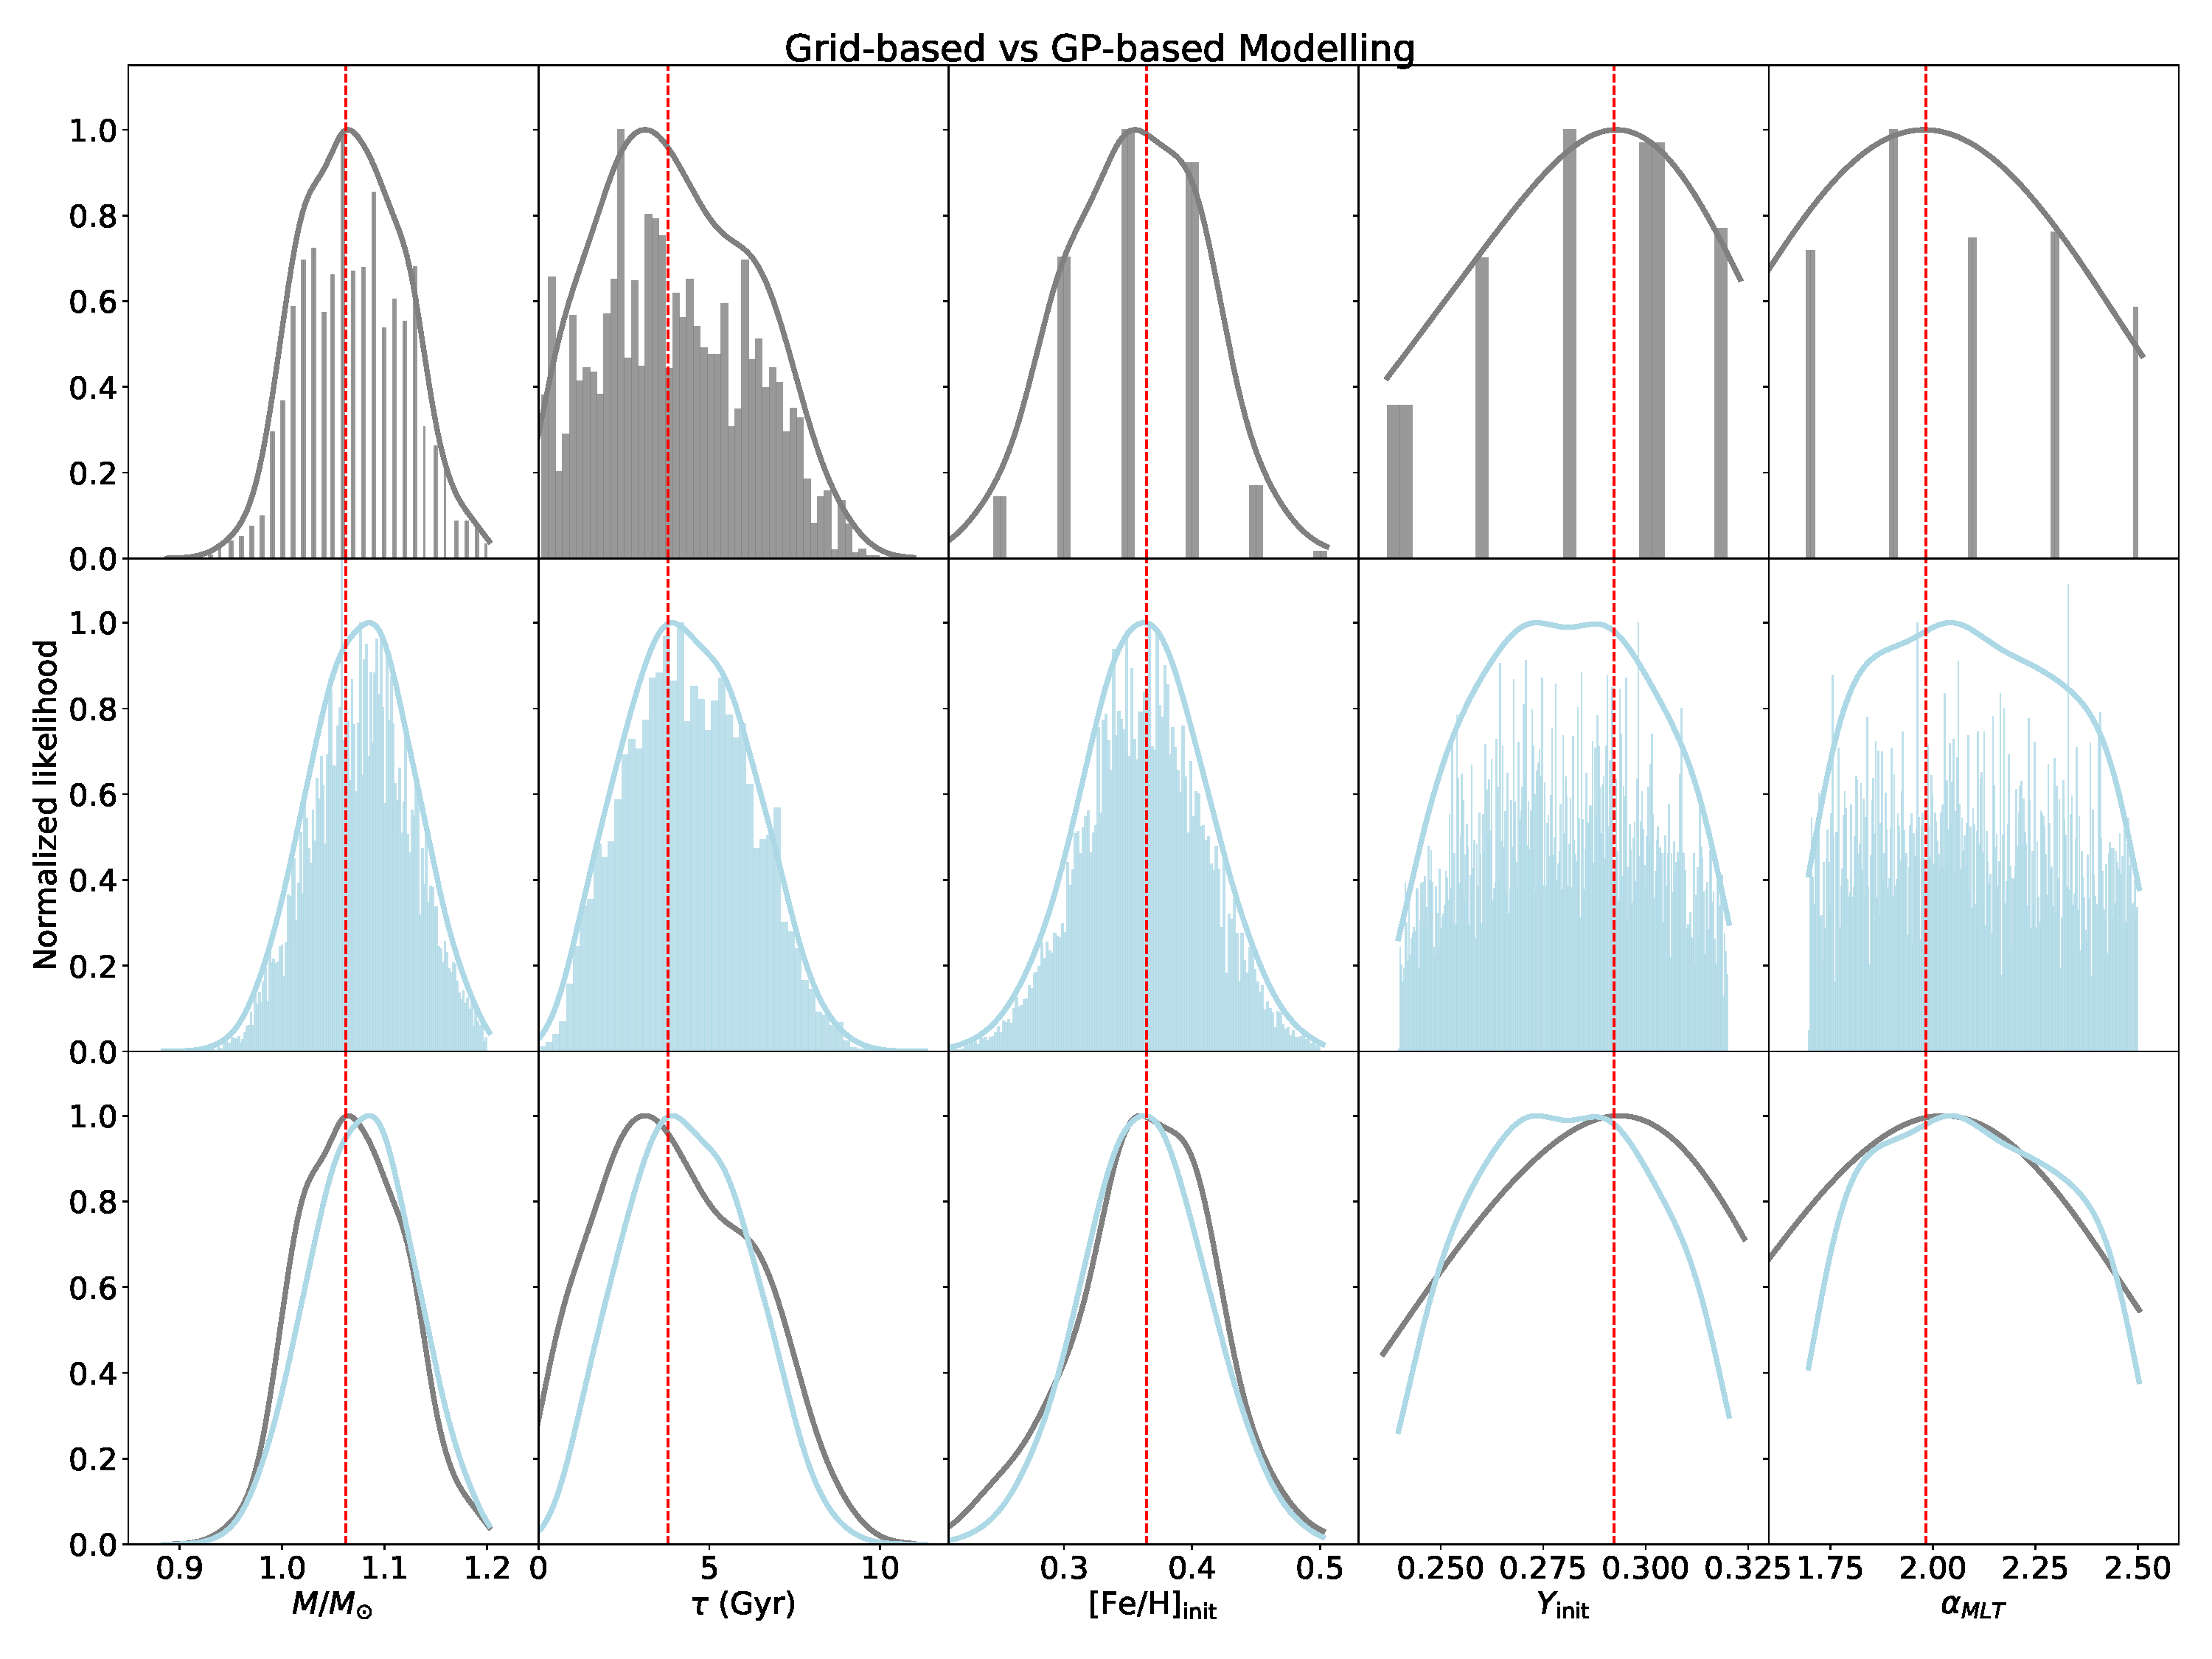
\includegraphics[width=1.9\columnwidth]{gp_fitting.pdf}
    \caption{Probability distributions of five fundamental parameters from grid-based (top row) and GP-based modelling (middle row) for a fake star. Grey solid lines in the top row and blue solid lines in the middle row are the kernel density of probability distributions. The bottom row demonstrates comparisons between kernel densities based on the two methods. True fundamental parameters, indicated by red dashed lines, are $M$ = 1.062$\rm M_{\odot}$, $\tau$ = 3.79Gyr, $\rm {\it [Fe/H]}_{init}$ = 0.364, $Y_{\rm init}$ = 0.292, and $\alpha_{\rm MLT}$ = 1.984. Observed constraints for this fake star are $T_{\rm eff}$ = 5652$\pm$50K, $\log g$ = 4.424$\pm$0.005, {\it [Fe/H]}$_{\rm surf}$ =  0.31$\pm$0.05, and $R$ =  1.047$\pm$0.031$R_{\odot}$. } 
  \label{fig:fit_comparison}
\end{figure*}

We compared estimates for the 1,000 fake stars and find remarkable improvements in GP-based modelling. 
The average precisions are 4.7\% for mass and 26\% for age with the original grid and 4.5\%and 19\% with GP predictions. 
%
The accuracy of GP-based modelling is examined as illustrated in Figure \ref{fig:fake_test}, in which we compare modelling solutions with fake stars'  true masses and ages.
Good consistence is found, and we also see that differences nicely follow a normal distribution, saying that the fitting is only affected by random noises in observations. 
%
Comparing between grid-based and GP-based modelling, their results for the mass both consist with truths, but the median age difference shifts to around -0.2 for the grid-based modelling. This corresponds to what is seen in Figure \ref{fig:fit_comparison}, that the grid-based modelling can underestimate the age because of the in-completed sampling. We hence conclude that GP-based modelling can better recover stellar properties.

\begin{figure*}
	%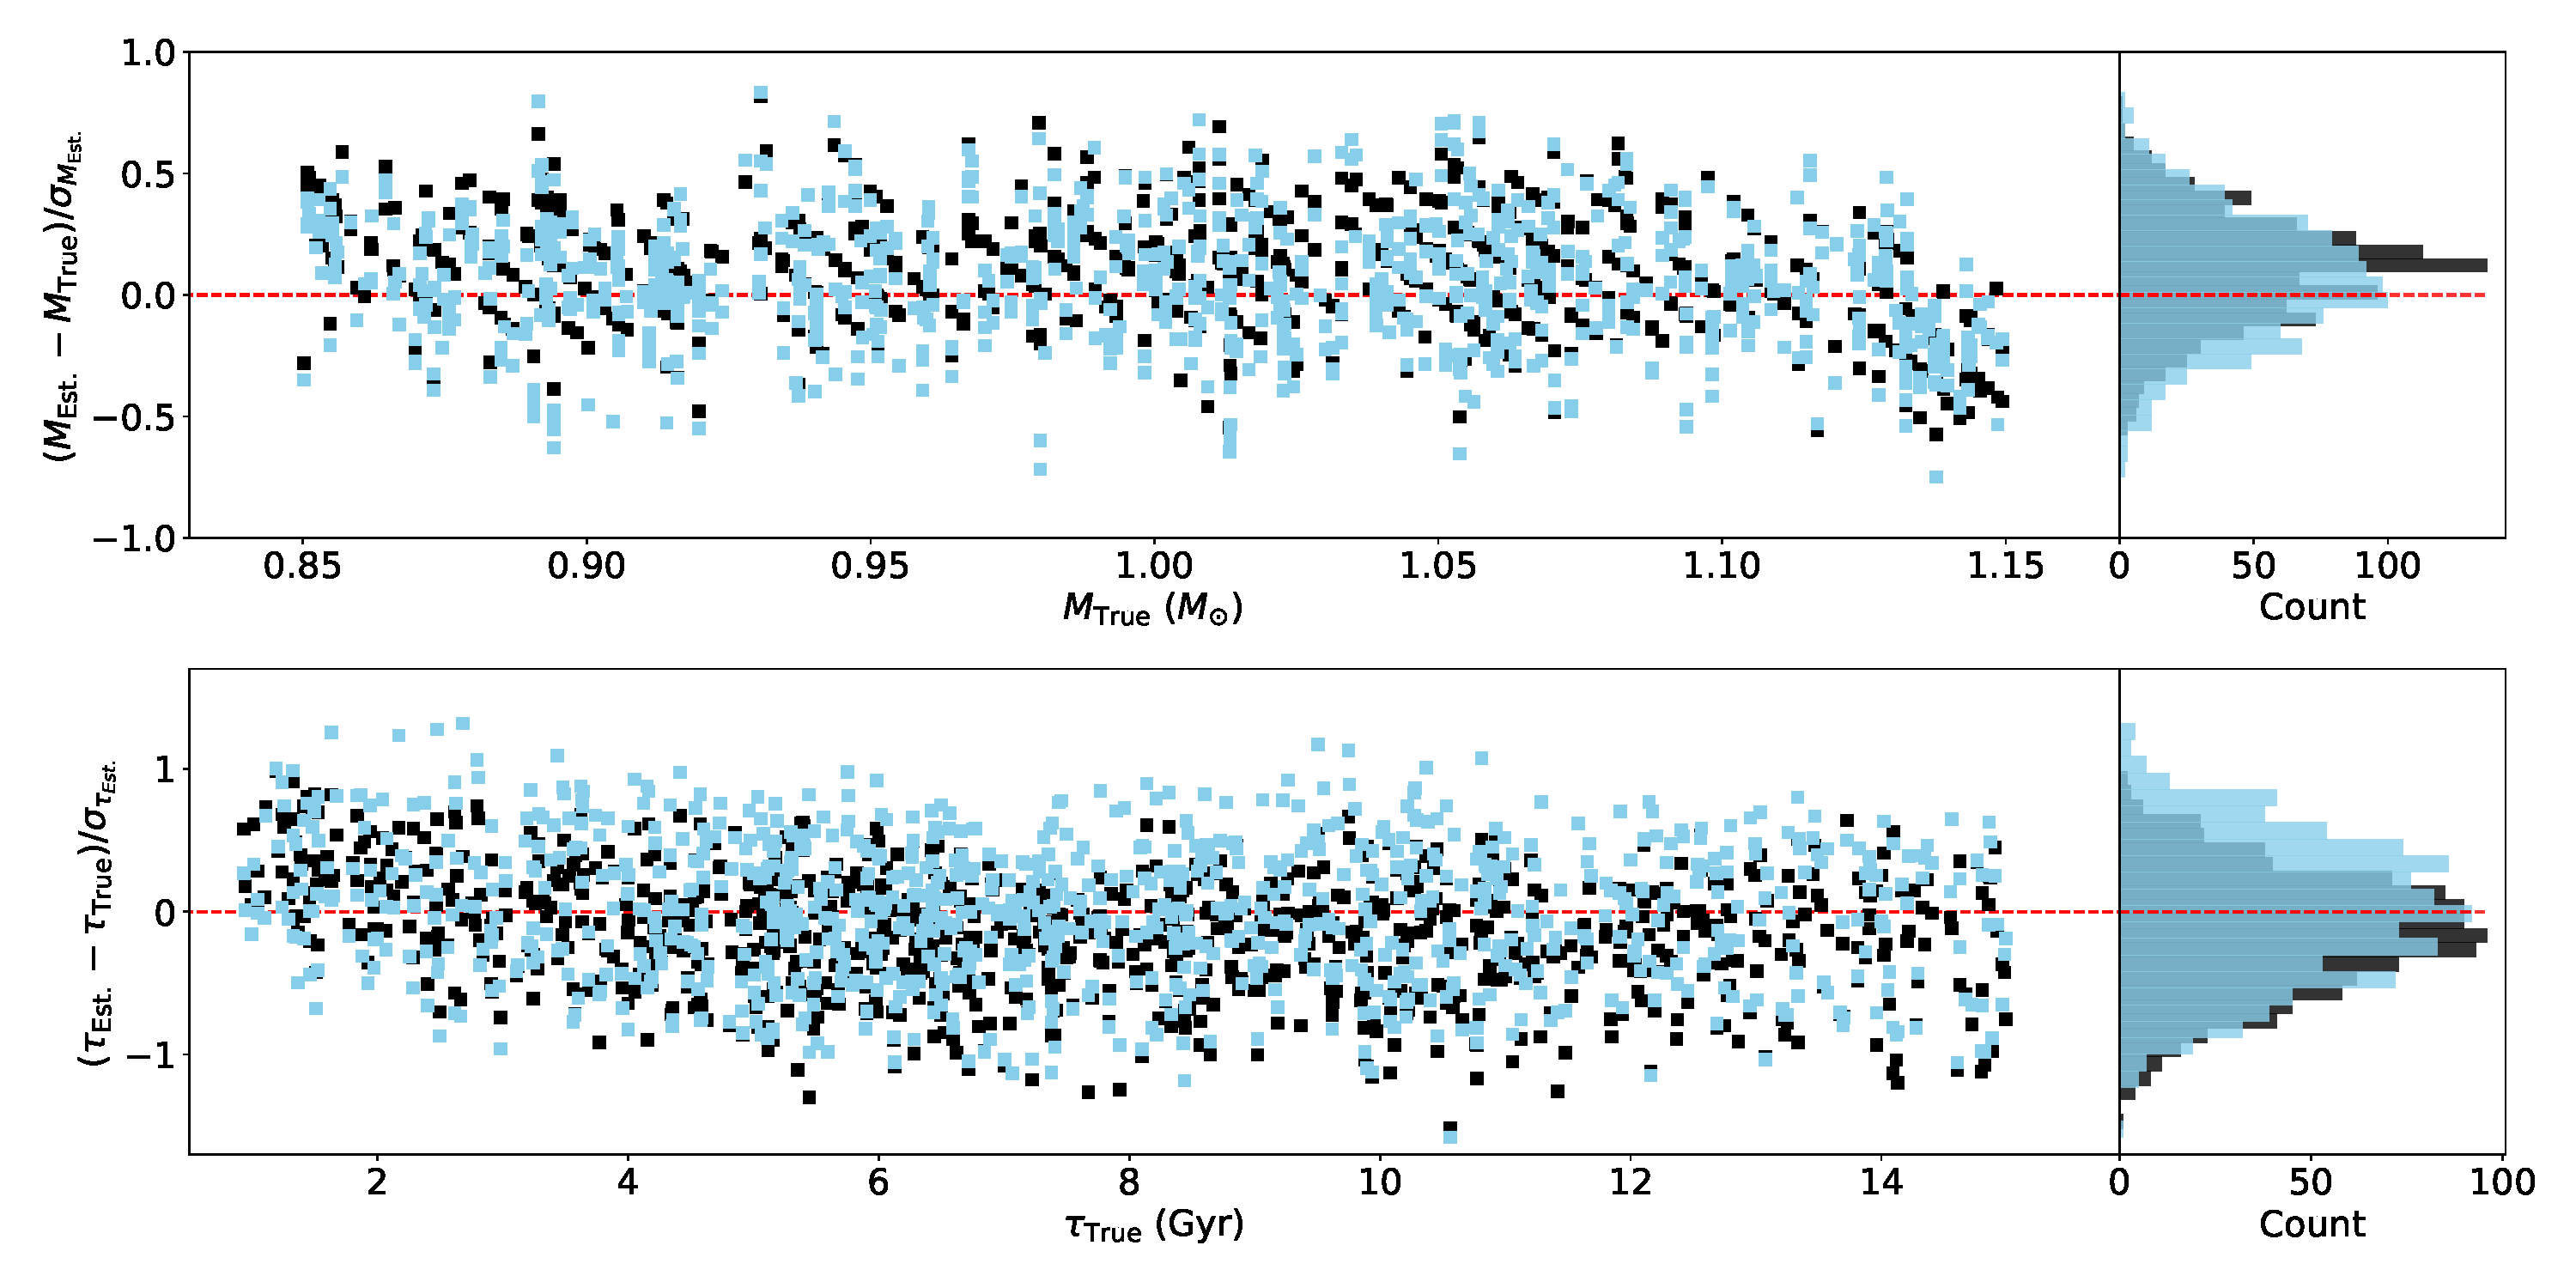
\includegraphics[width=1.8\columnwidth]{fake-stars-test.pdf}
	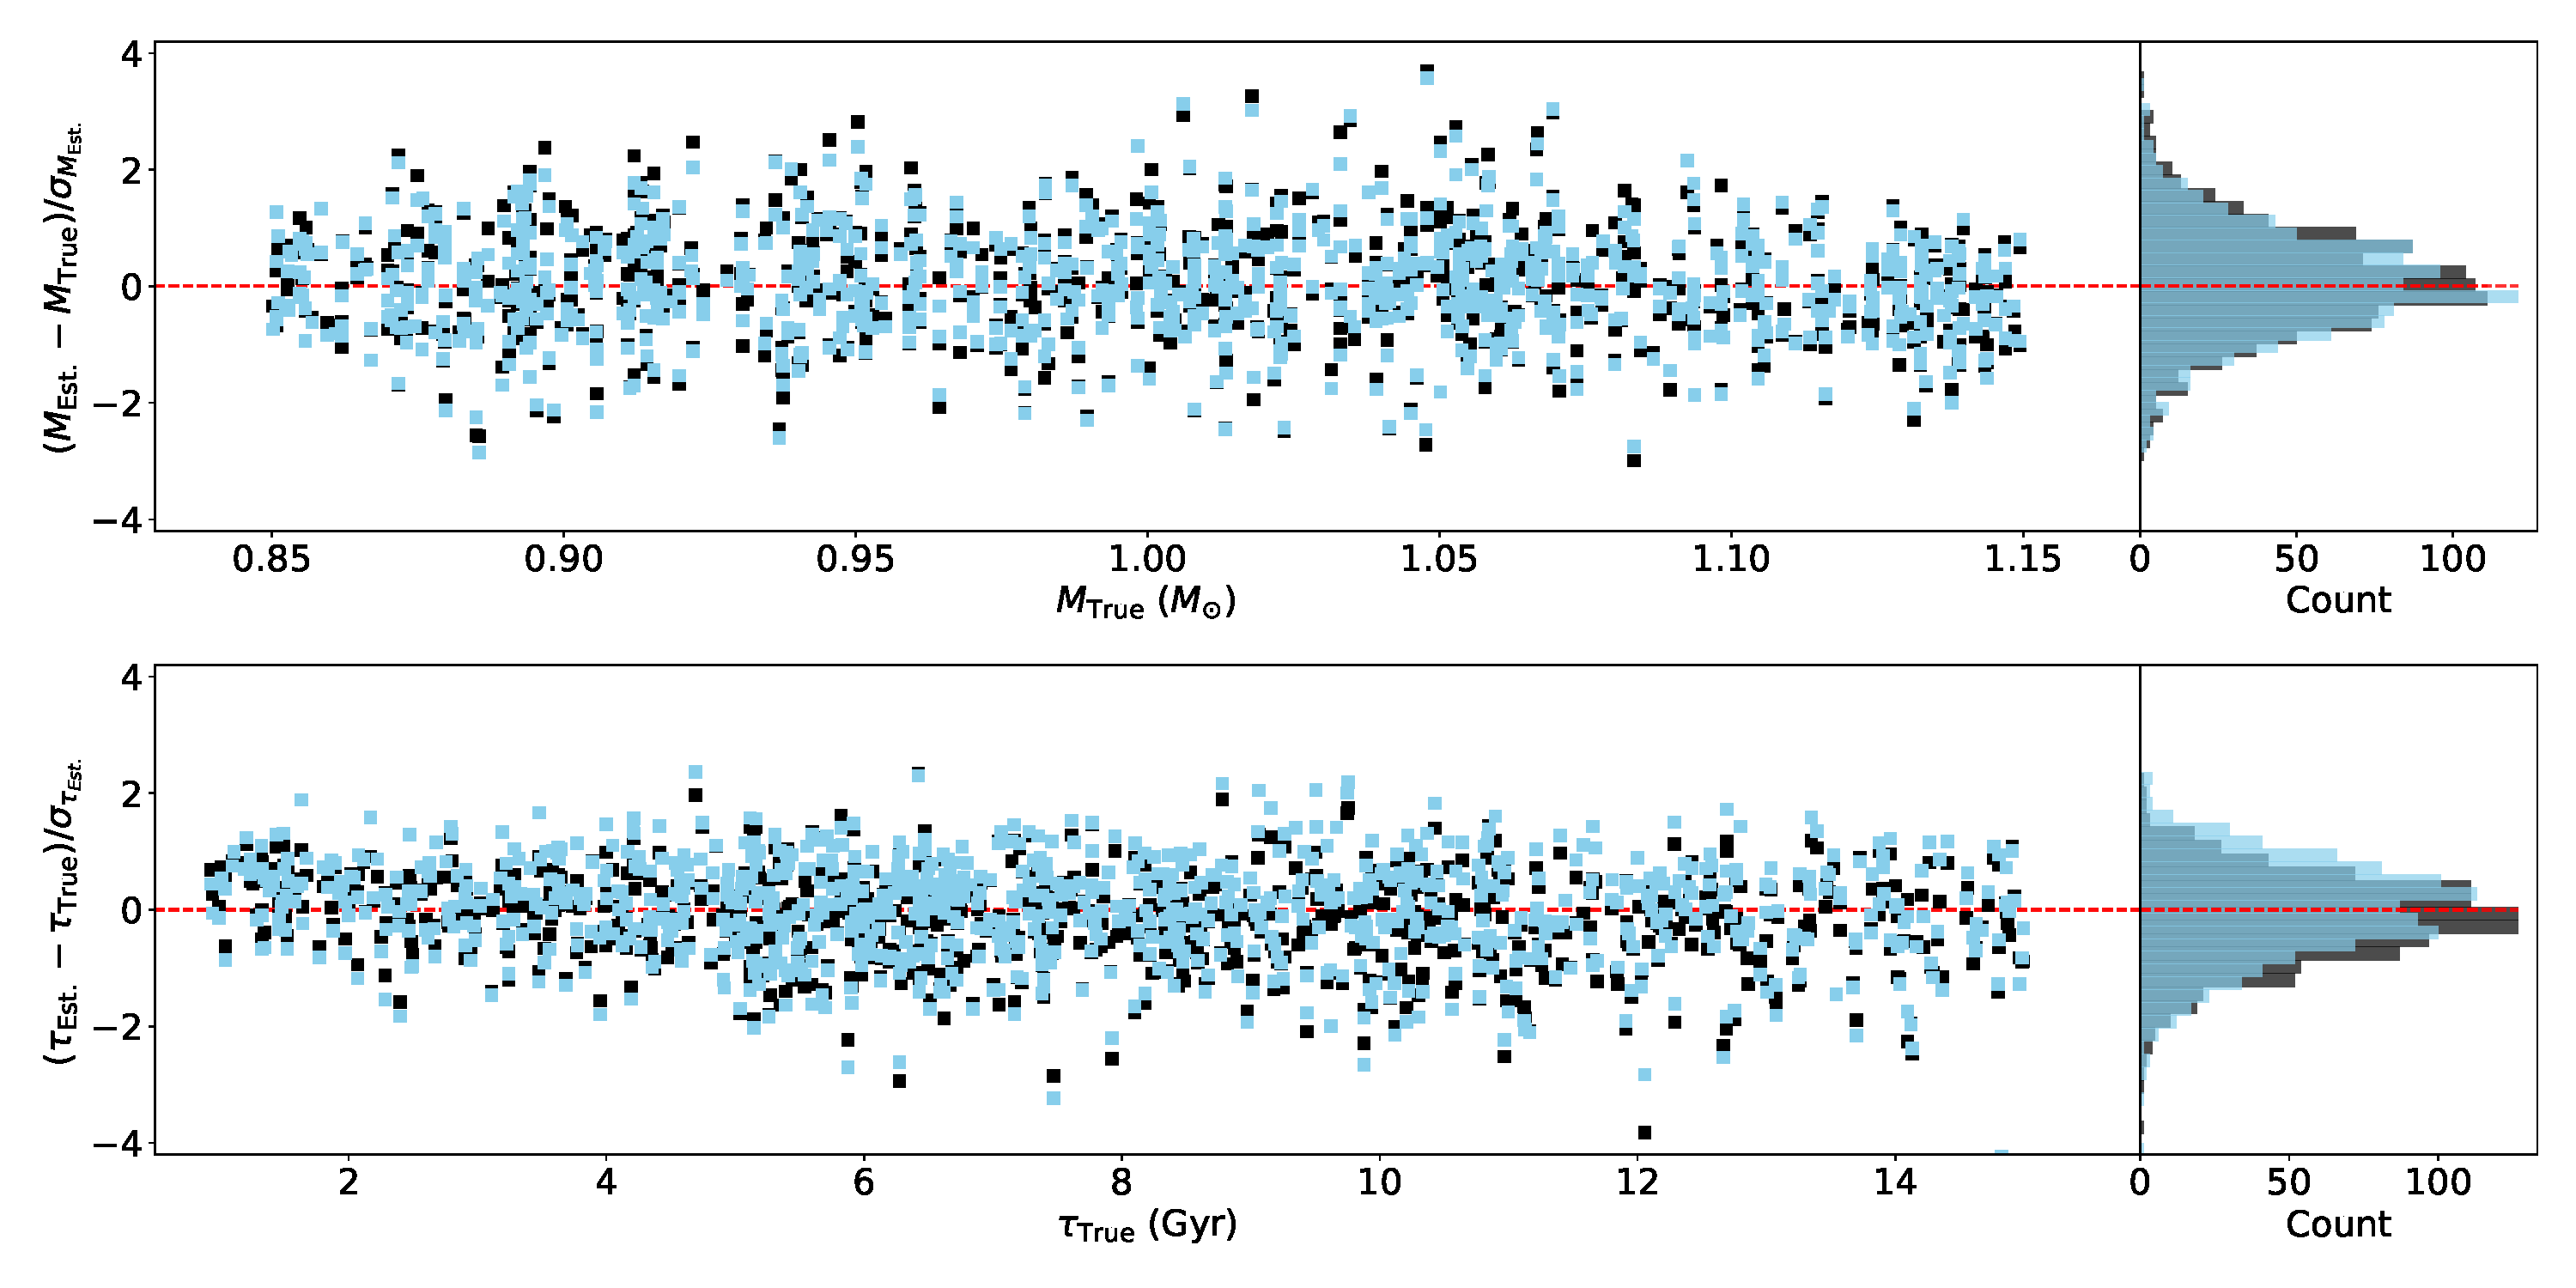
\includegraphics[width=1.8\columnwidth]{fake-stars-test-2.pdf}
    \caption{Differences between true and estimated stellar masses and ages over their estimated uncertainty of 1,000 fake stars. Black and blue symbols represent inferences with the original grid and with GP predictions. Count distributions of offsets are demonstrated on the right side.} 
  \label{fig:fake_test}
\end{figure*}









